%-------------------------------------------------------------------------

\documentclass[a4paper,twoside,11pt]{article}
\usepackage{a4wide}
\usepackage{graphicx}
\usepackage{fancyhdr}
\usepackage{clrscode}
\usepackage{tabularx}
\usepackage{amsmath}
\usepackage{amssymb}
\usepackage{xcolor}
\usepackage{enumitem}
\usepackage{hyperref}
\usepackage{indentfirst}
\graphicspath{ {./images/} }

%----------------------- Macros and Definitions --------------------------

\setlength\headheight{20pt}
\addtolength\topmargin{-10pt}
\addtolength\footskip{20pt}
\numberwithin{equation}{section}

\fancypagestyle{plain}{%
\fancyhf{}
\fancyhead[LO,RE]{\sffamily ETH Zürich}
\fancyhead[RO,LE]{\sffamily Model Predictive Control}
\fancyfoot[LO,RE]{\sffamily /D-MAVT}
\fancyfoot[RO,LE]{\sffamily\bfseries\thepage}
\renewcommand{\headrulewidth}{0pt}
\renewcommand{\footrulewidth}{0pt}
}

\pagestyle{fancy}
\fancyhf{}
\fancyhead[RO,LE]{\sffamily Model Predictive Control}
\fancyhead[LO,RE]{\sffamily ETH Zürich}
\fancyfoot[LO,RE]{\sffamily /D-MAVT}
\fancyfoot[RO,LE]{\sffamily\bfseries\thepage}
\renewcommand{\headrulewidth}{1pt}
\renewcommand{\footrulewidth}{0pt}

\definecolor{ORANGE}{rgb}{0.85, 0.33, 0.1}
\definecolor{GREEN}{rgb}{0.47, 0.67, 0.1}
\definecolor{RED}{rgb}{0.64, 0.08, 0.1}
\definecolor{PURPLE}{rgb}{0.49, 0.18, 0.5}

%--------------------------- Document --------------------------------

\begin{document}

\begin{titlepage}
    \begin{center}
        \vspace*{5cm}
        
        \includegraphics[width=0.4\textwidth]{logo/eth.eps}
        
        \vspace*{1cm}
        
        \huge
        \textbf{Model Predictive Control}
        
        \LARGE
        \textbf{Programming Exercise Report}
            
        \vspace*{1cm}
        
        \vfill
        
        \large
        \today
        
        \vspace*{1cm}
        
        \large
        \textbf{Chenhao Li} \quad 20-953-139 \quad \href{mailto:chenhli@student.ethz.ch}{\text{chenhli@student.ethz.ch}}
        
        \textbf{Jin Cheng} \quad 20-946-158 \quad \href{mailto:jicheng@student.ethz.ch}{\text{jicheng@student.ethz.ch}}
        
        \textbf{Yidan Gao} \quad 20-952-792 \quad \href{mailto:yidgao@student.ethz.ch}{\text{yidgao@student.ethz.ch}}
        

    \end{center}
\end{titlepage}

\pagenumbering{roman}
\tableofcontents

\newpage

%----------------------------------------------------------------
\pagenumbering{arabic}
\section{System Modeling}

\subsection{Task 1: Continuous-time State-space Description (2 pt.)} 
 
The system dynamics can be written as
\begin{equation}
\begin{split}
    m_{VC}\dot{T}^c_{VC}(t) & = (-\alpha_{F1,VC}-\alpha_{F2,VC}-\alpha_{Env,VC})T^c_{VC}(t) \\ 
                            & + \alpha_{F1,VC}T^c_{F1}(t) \\
                            & + \alpha_{F2,VC}T^c_{F2}(t) \\
                            & + \beta_{11}p^c_{VC}(t) + \beta_{12}p^c_{F1}(t) + \beta_{13}p^c_{F2}(t) \\
                            & + \alpha_{Env,VC}T_{Env} + d_{vc}
\end{split}
\end{equation}
\begin{equation}
\begin{split}
    m_{F1}\dot{T}^c_{F1}(t) & = \alpha_{VC,F1}T^c_{VC}(t) \\
                            & + (-\alpha_{VC,F1}-\alpha_{F2,F1})T^c_{F1}(t) \\
                            & + \alpha_{F2,F1}T^c_{F2}(t) \\
                            & + \beta_{21}p^c_{VC}(t) + \beta_{22}p^c_{F1}(t) + \beta_{23}p^c_{F2}(t) \\
                            & + d_{F1}
\end{split}
\end{equation}
\begin{equation}
\begin{split}
    m_{F2}\dot{T}^c_{F2}(t) & = \alpha_{VC,F2}T^c_{VC}(t) \\
                            & + \alpha_{F1,F2}T^c_{F1}(t) \\
                            & + (-\alpha_{VC,F2}-\alpha_{F1,F2})T^c_{F2}(t) \\
                            & + \beta_{31}p^c_{VC}(t) + \beta_{32}p^c_{F1}(t) + \beta_{33}p^c_{F2}(t) \\
                            & + d_{F2}
\end{split}
\end{equation}

We could reorganize it in the continuous-time state-space description
\begin{equation}
    \dot{T}^c(t) = A^cT^c(t) + B^cp^c(t) + B^c_d d^c
\end{equation}
where 
\begin{equation*}
\begin{split}
    \dot{T}^c(t) &= 
    \begin{bmatrix}
    \dot{T}^c_{VC}(t)\\
    \dot{T}^c_{F1}(t)\\
    \dot{T}^c_{F2}(t)
    \end{bmatrix}
    , 
    T^c(t) = 
    \begin{bmatrix}
    T^c_{VC}(t)\\
    T^c_{F1}(t)\\
    T^c_{F2}(t)
    \end{bmatrix}
    , \\
    p^c(t) &= 
    \begin{bmatrix}
    p^c_{VC}(t)\\
    p^c_{F1}(t)\\
    p^c_{F2}(t)
    \end{bmatrix}
    , 
    d^c = 
    \begin{bmatrix}
    d^c_{VC}\\
    d^c_{F1}\\
    d^c_{F2}
    \end{bmatrix}
    =
    \begin{bmatrix}
    \alpha_{Env,VC}T_{Env} + d_{VC}\\
    d_{F1}\\
    d_{F2}
    \end{bmatrix}
\end{split}
\end{equation*}
and
\begin{equation*}
\begin{split}
    A^c &= 
    \begin{bmatrix}
    -\frac{\alpha_{F1,VC}+\alpha_{F2,VC}+\alpha_{Env,VC}}{m_{VC}} & \frac{\alpha_{F1,VC}}{m_{VC}} & \frac{\alpha_{F2,VC}}{m_{VC}} \\
    \frac{\alpha_{VC,F1}}{m_{F1}} & -\frac{\alpha_{VC,F1}+\alpha_{F2,F1}}{m_{F1}} & \frac{\alpha_{F2,F1}}{m_{F1}} \\
    \frac{\alpha_{VC,F2}}{m_{F2}} & \frac{\alpha_{F1,F2}}{m_{F2}} & -\frac{\alpha_{VC,F2}+\alpha_{F1,F2}}{m_{F2}}
    \end{bmatrix} \\
    &=
    \begin{bmatrix}
    -8.6310\times10^{-5} & 5.3571\times10^{-6} & 9.5238\times10^{-6}\\
    5.7692\times10^{-5} & -2.3333\times10^{-4} & 1.7564\times10^{-4}\\
    3.0769\times10^{-4} & 5.2692\times10^{-4} & -8.3462\times10^{-4}
    \end{bmatrix}
\end{split}
\end{equation*}
\begin{equation*}
\begin{split}
    B^c &= 
    \begin{bmatrix}
    \frac{\beta_{11}}{m_{VC}} & \frac{\beta_{12}}{m_{VC}} & \frac{\beta_{13}}{m_{VC}} \\
    \frac{\beta_{21}}{m_{F1}} & \frac{\beta_{22}}{m_{F1}} & \frac{\beta_{23}}{m_{F1}} \\
    \frac{\beta_{31}}{m_{F2}} & \frac{\beta_{32}}{m_{F2}} & \frac{\beta_{33}}{m_{F2}} 
    \end{bmatrix} \\
    &=
    \begin{bmatrix}
    1.9048\times10^{-7} & -1.1905\times10^{-8} & -1.1905\times10^{-8}\\
    2.5641\times10^{-7} & 2.0513\times10^{-6} & 1.2821\times10^{-7}\\
    7.6923\times10^{-7} & 1.1538\times10^{-6} & 6.9231\times10^{-6}
    \end{bmatrix}
\end{split}
\end{equation*}
\begin{equation*}
\begin{split}
     B^c_d &= 
    \begin{bmatrix}
    \frac{1}{m_{VC}} & 0 & 0 \\
    0 & \frac{1}{m_{F1}} & 0 \\
    0 & 0 & \frac{1}{m_{F2}} 
    \end{bmatrix} \\
    &=
    \begin{bmatrix}
    2.3810\times10^{-7} & 0 & 0 \\
    0 & 2.5641\times10^{-6} & 0 \\
    0 & 0 & 7.6923\times10^{-6} \\
    \end{bmatrix} \\
\end{split}
\end{equation*}
   
\subsection{Task 2: Discrete-time State-space Description (3 pt.)}

We can approximate 
\begin{equation}
    \dot{T}^c(kT_s) \approx \frac{T^c(kT_s+T_s) - T^c(kT_s)}{T_s} = \frac{T(k+1)-T(k)}{T_s}
\end{equation}
such that $T(k) = T^c(kT_s)$. Also, we have $T(0) = T^c(0)$.

By plugging the approximation in the system dynamics we could discretize the system as followed
\begin{equation}
    T(k+1) = AT(k)+Bp(k)+B_dd
\end{equation}
where 
\begin{equation*}
    T(k) = 
    \begin{bmatrix}
    T_{VC}(k)\\
    T_{F1}(k)\\
    T_{F2}(k)
    \end{bmatrix}
    , 
    p(k) = 
    \begin{bmatrix}
    p_{VC}(k)\\
    p_{F1}(k)\\
    p_{F2}(k)
    \end{bmatrix}
    , 
    d = d^c = 
    \begin{bmatrix}
    \alpha_{Env,VC}T_{Env} + d_{vc}\\
    d_{F1}\\
    d_{F2}
    \end{bmatrix}
\end{equation*}
and
\begin{equation*}
\begin{split}
    A &= 
    T_sA^c + I \\
    &= 
    \begin{bmatrix}
    1-\frac{\alpha_{F1,VC}+\alpha_{F2,VC}+\alpha_{Env,VC}}{m_{VC}}T_s & \frac{\alpha_{F1,VC}}{m_{VC}}T_s & \frac{\alpha_{F2,VC}}{m_{VC}}T_s \\
    \frac{\alpha_{VC,F1}}{m_{F1}}T_s & 1-\frac{\alpha_{VC,F1}+\alpha_{F2,F1}}{m_{F1}}T_s & \frac{\alpha_{F2,F1}}{m_{F1}}T_s \\
    \frac{\alpha_{VC,F2}}{m_{F2}}T_s & \frac{\alpha_{F1,F2}}{m_{F2}}T_s & 1-\frac{\alpha_{VC,F2}+\alpha_{F1,F2}}{m_{F2}}T_s
    \end{bmatrix} \\
    &=
    \begin{bmatrix}
    0.9948 & 3.2143\times10^{-4} & 5.7143\times10^{-4} \\
    0.0035 & 0.9860 & 0.0105 \\
    0.0185 & 0.0316 & 0.9499 
    \end{bmatrix}
\end{split}
\end{equation*}
\begin{equation*}
\begin{split}
    B &= 
    T_sB^c \\
    &= 
    \begin{bmatrix}
    \frac{\beta_{11}}{m_{VC}}T_s & \frac{\beta_{12}}{m_{VC}}T_s & \frac{\beta_{13}}{m_{VC}}T_s \\
    \frac{\beta_{21}}{m_{F1}}T_s & \frac{\beta_{22}}{m_{F1}}T_s & \frac{\beta_{23}}{m_{F1}}T_s \\
    \frac{\beta_{31}}{m_{F2}}T_s & \frac{\beta_{32}}{m_{F2}}T_s & \frac{\beta_{33}}{m_{F2}}T_s 
    \end{bmatrix}\\
    &=
    \begin{bmatrix}
    1.1429\times10^{-5} & -7.1429\times10^{-7} & -7.1429\times10^{-7} \\ 
    1.5385\times10^{-5} & 1.2308\times10^{-4} & 7.6923\times10^{-6} \\
    4.6154\times10^{-5} & 6.9231\times10^{-5} & 4.1538\times10^{-4}
    \end{bmatrix}
\end{split}
\end{equation*}
\begin{equation*}
\begin{split}
    B_d &= 
    T_sB_d^c \\
    &= 
    \begin{bmatrix}
    \frac{1}{m_{VC}}T_s & 0 & 0 \\
    0 & \frac{1}{m_{F1}}T_s & 0 \\
    0 & 0 & \frac{1}{m_{F2}}T_s 
    \end{bmatrix}\\
    &=
    \begin{bmatrix}
    1.4286\times10^{-5} & 0 & 0\\
    0 & 1.5385\times10^{-4} & 0\\
    0 & 0 & 4.6154\times10^{-4}
    \end{bmatrix}
\end{split}
\end{equation*}

\subsection{Task 3: Steady-state and Delta-Formulation (2 pt.)}

Using the steady-state condition, we have
\begin{equation}
    T_{sp} = T_{Target}
\end{equation}
\begin{equation}
    T_{sp} = AT_{sp}+Bp_{sp}+B_dd
\end{equation}
where $T_{Target} = [25, -42, -18.5]^\top$

By solving the equation, we can get the steady-state and the corresponding input
\begin{equation*}
    T_{sp} = 
    \begin{bmatrix}
    25 \\
    -42 \\
    -18.5
    \end{bmatrix}
    , \quad
    p_{sp} = 
    \begin{bmatrix}
    8.2373\times10^{3} \\
    -4.9111\times10^{3} \\
    -241.4589
    \end{bmatrix}
\end{equation*}

The corresponding Delta-Formulation is 
\begin{equation}
    \Delta T(k+1) = A \Delta T(k) + B \Delta p(k)
\end{equation}
where
\begin{equation*}
    \Delta T(k) = T(k) - T_{sp} = 
    \begin{bmatrix}
    T_{VC}(k) - 25\\
    T_{F1}(k) + 42\\
    T_{F2}(k) + 18.5
    \end{bmatrix}
\end{equation*}

\begin{equation*}
    \Delta p(k) = p(k) - p_{sp} = 
    \begin{bmatrix}
    p_{VC}(k) - 8.2373\times10^{3}\\
    p_{F1}(k) + 4.9111\times10^{3}\\
    p_{F2}(k) + 241.4589
    \end{bmatrix}
\end{equation*}

\subsection{Task 4: Constraints (2 pt.)}

The constraints for the problem are
\begin{equation}
    \Delta T_{min} = 
    \begin{bmatrix}
    -3\\
    -3\\
    -0.5
    \end{bmatrix}
    \leq
    \Delta T(k) = 
    \begin{bmatrix}
    T_{VC}(k) - 25\\
    T_{F1}(k) + 42\\
    T_{F2}(k) + 18.5
    \end{bmatrix}
    \leq
    \begin{bmatrix}
    2\\
    3\\
    1.5
    \end{bmatrix}
     = \Delta T_{max}
\end{equation}
\begin{equation}
\begin{split}
    \Delta p_{min} = 
    \begin{bmatrix}
    -8.2373\times10^{3} \\
    -2.5889\times10^{3} \\
    -1.2585\times10^{3}
    \end{bmatrix}
    &\leq
    \Delta p(k) = 
    \begin{bmatrix}
    p_{VC}(k) - 8.2373\times10^{3}\\
    p_{F1}(k) + 4.9111\times10^{3}\\
    p_{F2}(k) + 241.4589
    \end{bmatrix}\\
    &\leq
    \begin{bmatrix}
    6.7627\times10^{3} \\
    4.9111\times10^{3} \\  
    241.4589
    \end{bmatrix}
     = \Delta p_{max}
\end{split}
\end{equation}

\newpage

%-----------------------------------------------------------

\section{Unconstrained Optimal Control}

\subsection{Task 5: Uncontrolled System (1 pt.)}

Figure \ref{fig:1} shows how the autonomous system (without any input) evolves with time. The temperature within the the building will drop below 22 \textdegree C in 40 minutes, while the temperature within both vaccinations will quickly increase and exceed the allowed maximum temperature in 20 minutes. 

\begin{figure}[h]
\centering
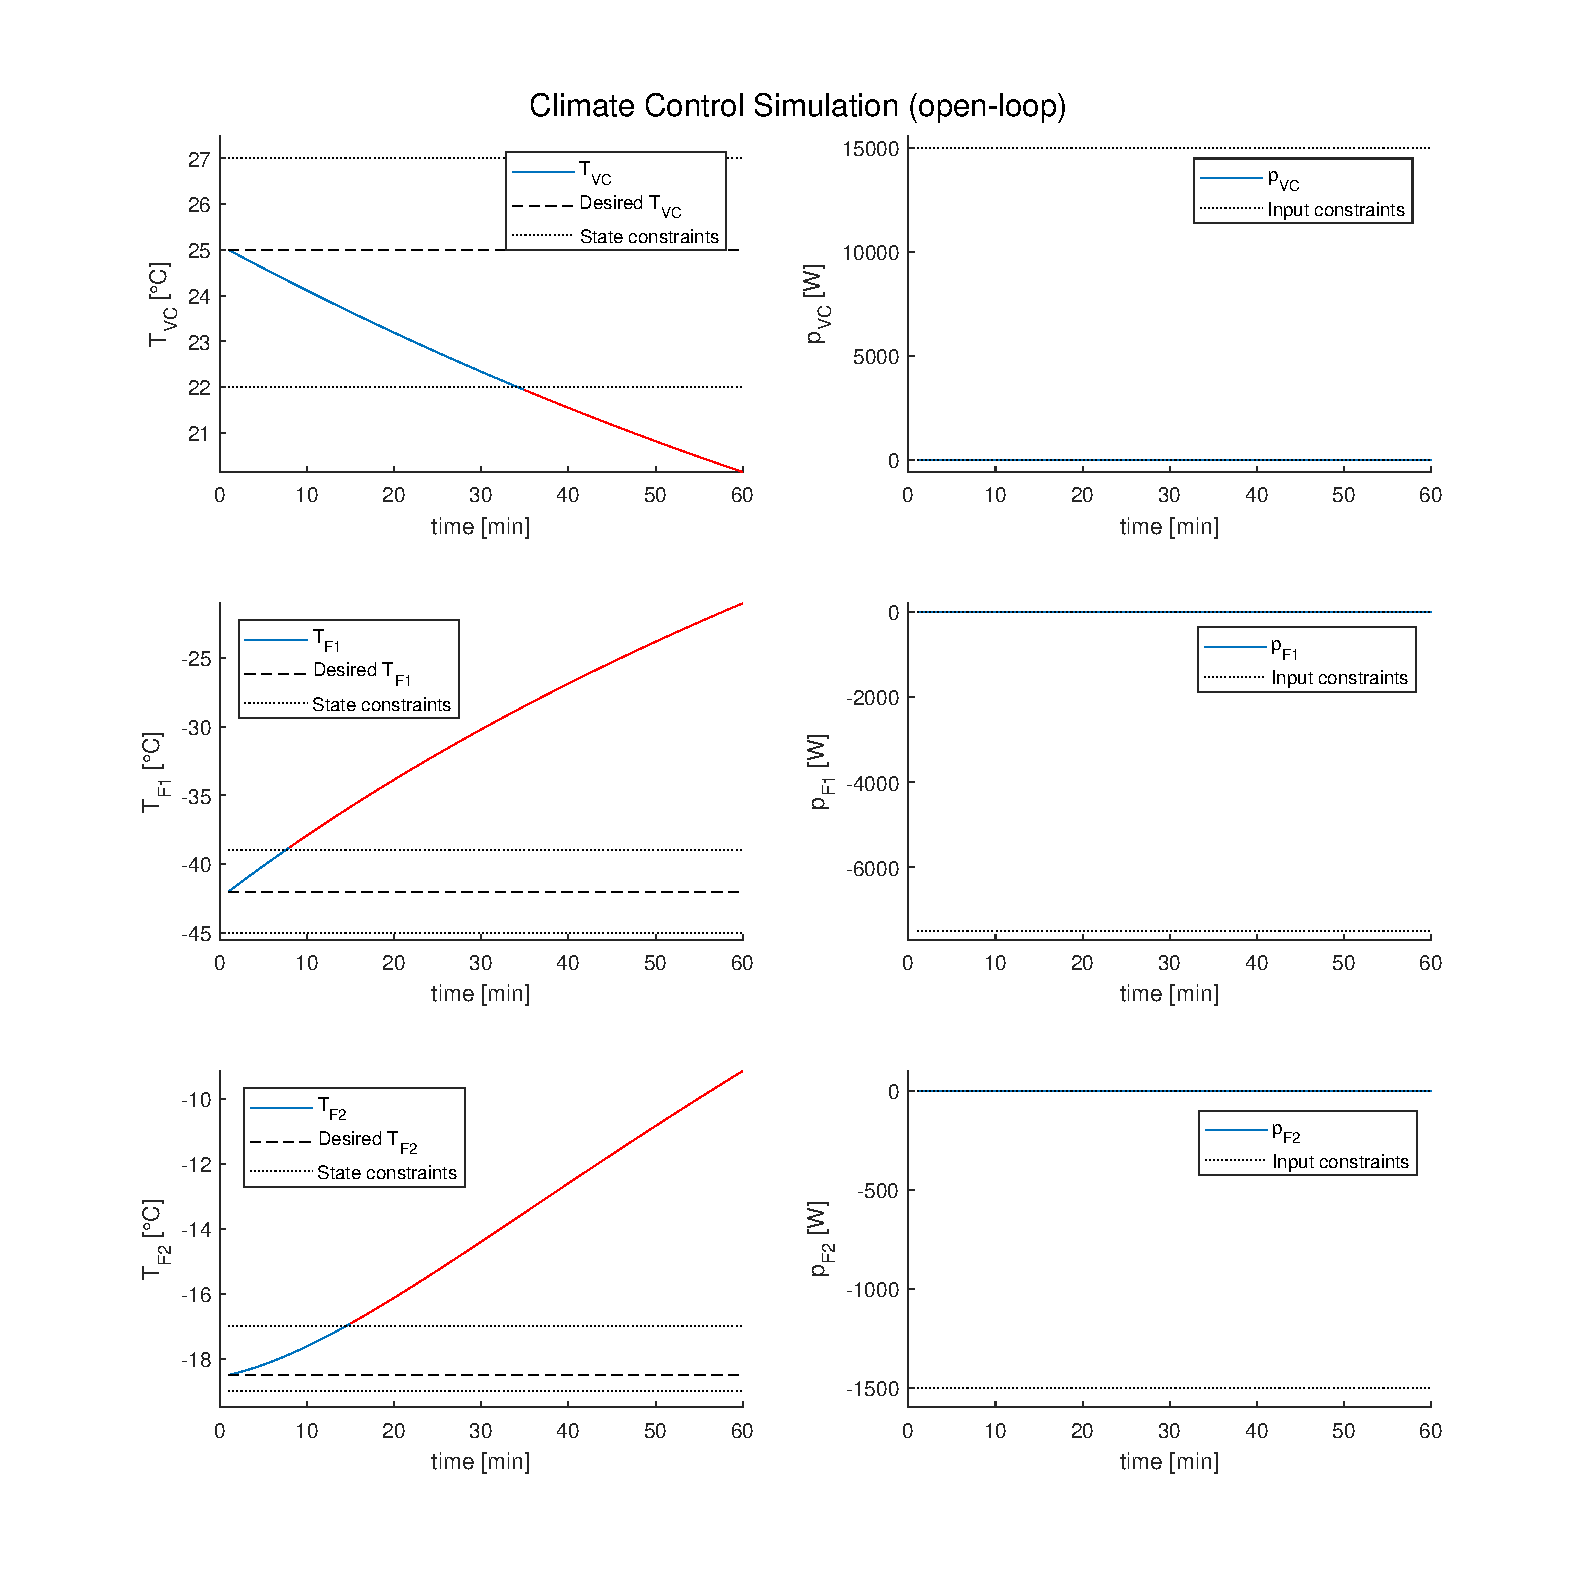
\includegraphics[scale = 0.58]{image/5.eps}
\caption{Uncontrolled system}
\label{fig:1}
\end{figure}

\subsection{Task 6: LQR Controller (4 pt.)}

Figure \ref{fig:2} shows the scatter plot, and the resulting $Q$ will take the value as followed.
\begin{equation*}
    Q = 
    \begin{bmatrix}
    4095905 & 0 & 0 \\
    0 & 2215882 & 0 \\
    0 & 0 & 1765919
    \end{bmatrix}
\end{equation*}

\begin{figure}[ht]
\centering
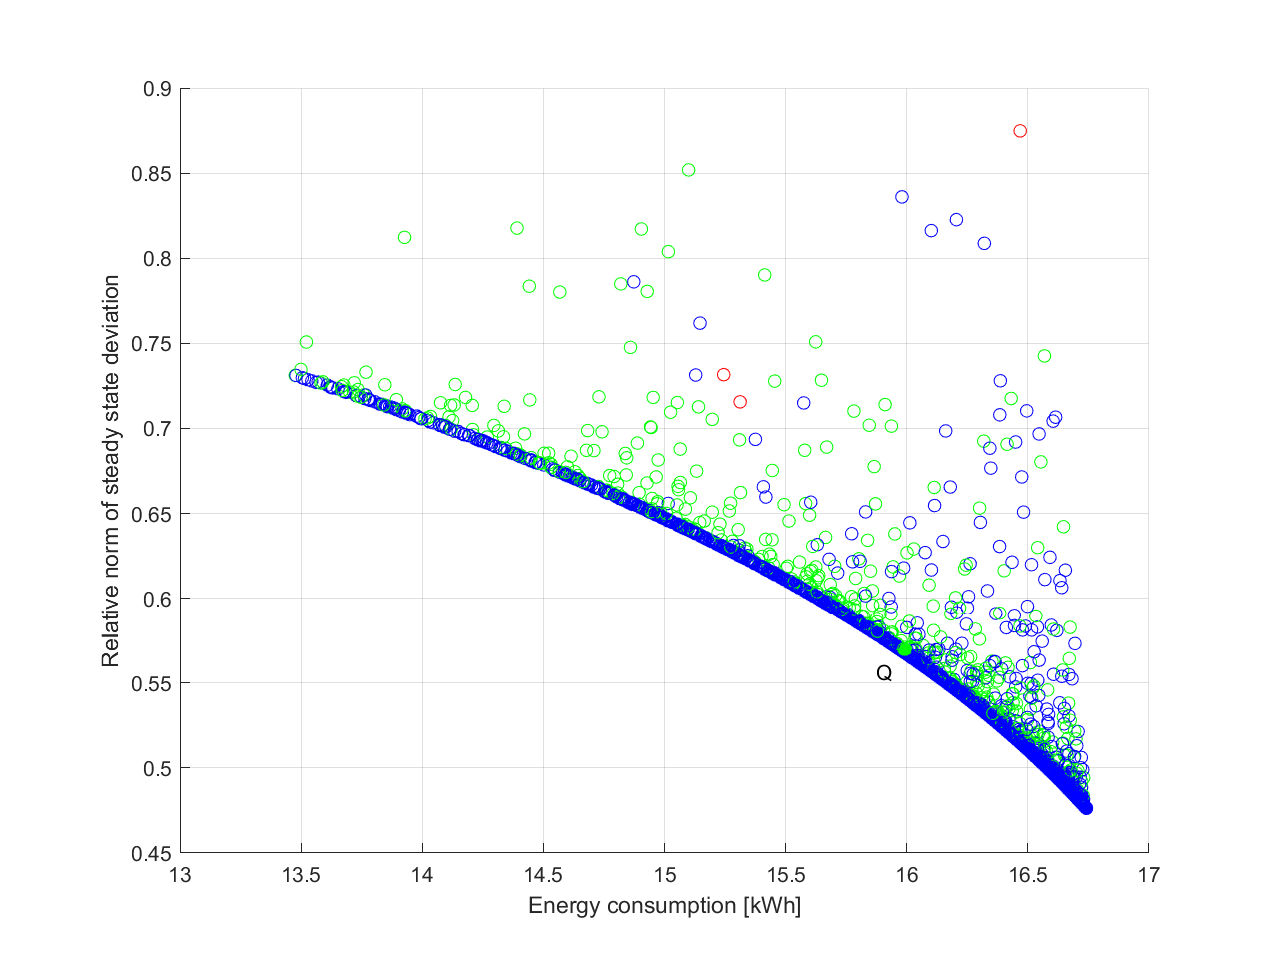
\includegraphics[scale = 0.7]{image/6.eps}
\caption{Heuristic LQR Tuning}
\label{fig:2}
\end{figure}

The scatter points lie in a specific range in the figure, which is $(13, 17)$ on energy consumption axis and $(0.45, 0.9)$ on relative norm of steady state deviation. 

From the figure, we can observe that for the $Q$s that violate the input constraints (marked blue), the energy consumption is negatively correlated with the relative norm of the steady state deviation, which means that for the whole system, we can only have a $Q$ that drives the state towards the steady state faster but consumes more energy in total, or vise versa. Since we put a constraint on energy consumption, the algorithm will search for a $Q$ that drives the system the relatively faster. Thus the resulting $Q$ (filled green point) will lie just around the energy consumption boundary. 

There are also a few blue data points above the curve, which scatter in the high-energy-consumption part (above 15 kWh). The reason for this is that for some larger $Q$s, the penalty for the state is too high that the system can only be driven by larger input, which consumes more energy. 

State constraints violation (marked red) happens rarely, which means that the proposed $Q$s can actually achieve a good performance to maintain the temperatures in the feasible range.

\subsection{Task 7: Simulation 1 with LQR Controller (2 pt.)}

\begin{figure}[ht]
\centering
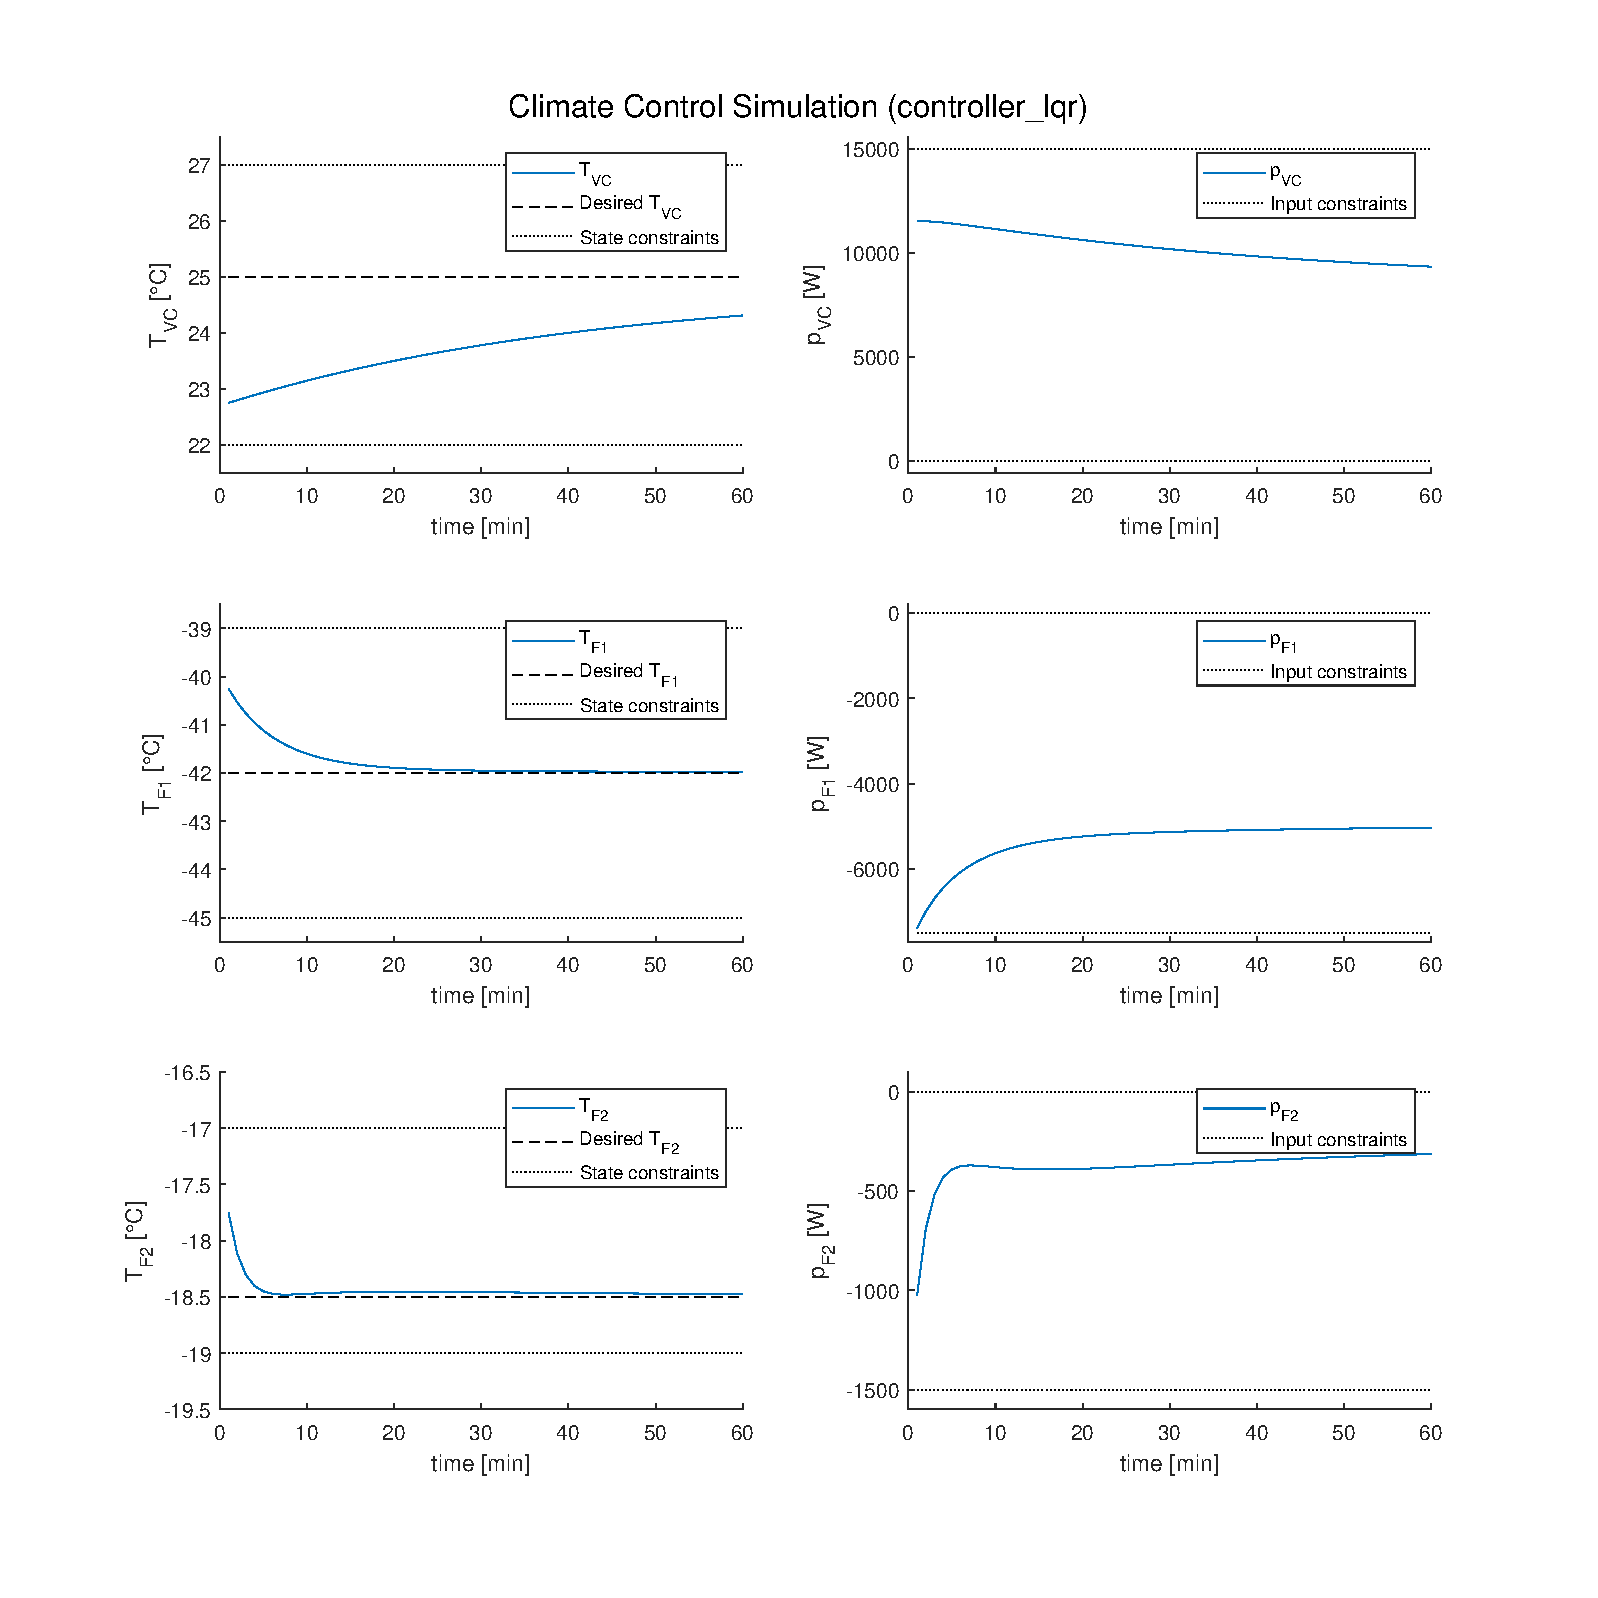
\includegraphics[scale = 0.58]{image/7.eps}
\caption{Simulation with initial condition 1 using LQR Controller}
\label{fig:3}
\end{figure}

Figure \ref{fig:3} shows the closed-loop simulation plot of the system under the LQR controller with the identity $R$ and the $Q$ found by the heuristic approach with the initial state $T(0) = T^{(1)}_{init} = T_{sp} + [-2.25 \ 1.75 \ 0.75]^\top$. 

We can observe that both of the vaccination temperatures will quickly be regulated to the ideal temperature, while the building temperature will not converge to the steady state even after 60 minutes. In comparison to the cooling units in the storing areas, which acts satisfactorily fast, the heating unit in the room changes slowly. 

What if we make changes on the diagonal elements in $Q$ and $R$? By increasing the diagonal values of $Q$, we will penalty more on the state (difference from the steady state) comparing to the input, which will result that the temperatures will converge faster to the steady state, while the system may increase its power as much as it could. On the contrary, if we increase $R$ and keep $Q$, we will penalty more on the input than the state. Thus, the input values will converge to the steady state input faster while the temperature will converge much slower.

\subsection{Task 8: Simulation 2 with LQR Controller (2 pt.)}

\begin{figure}[ht]
\centering
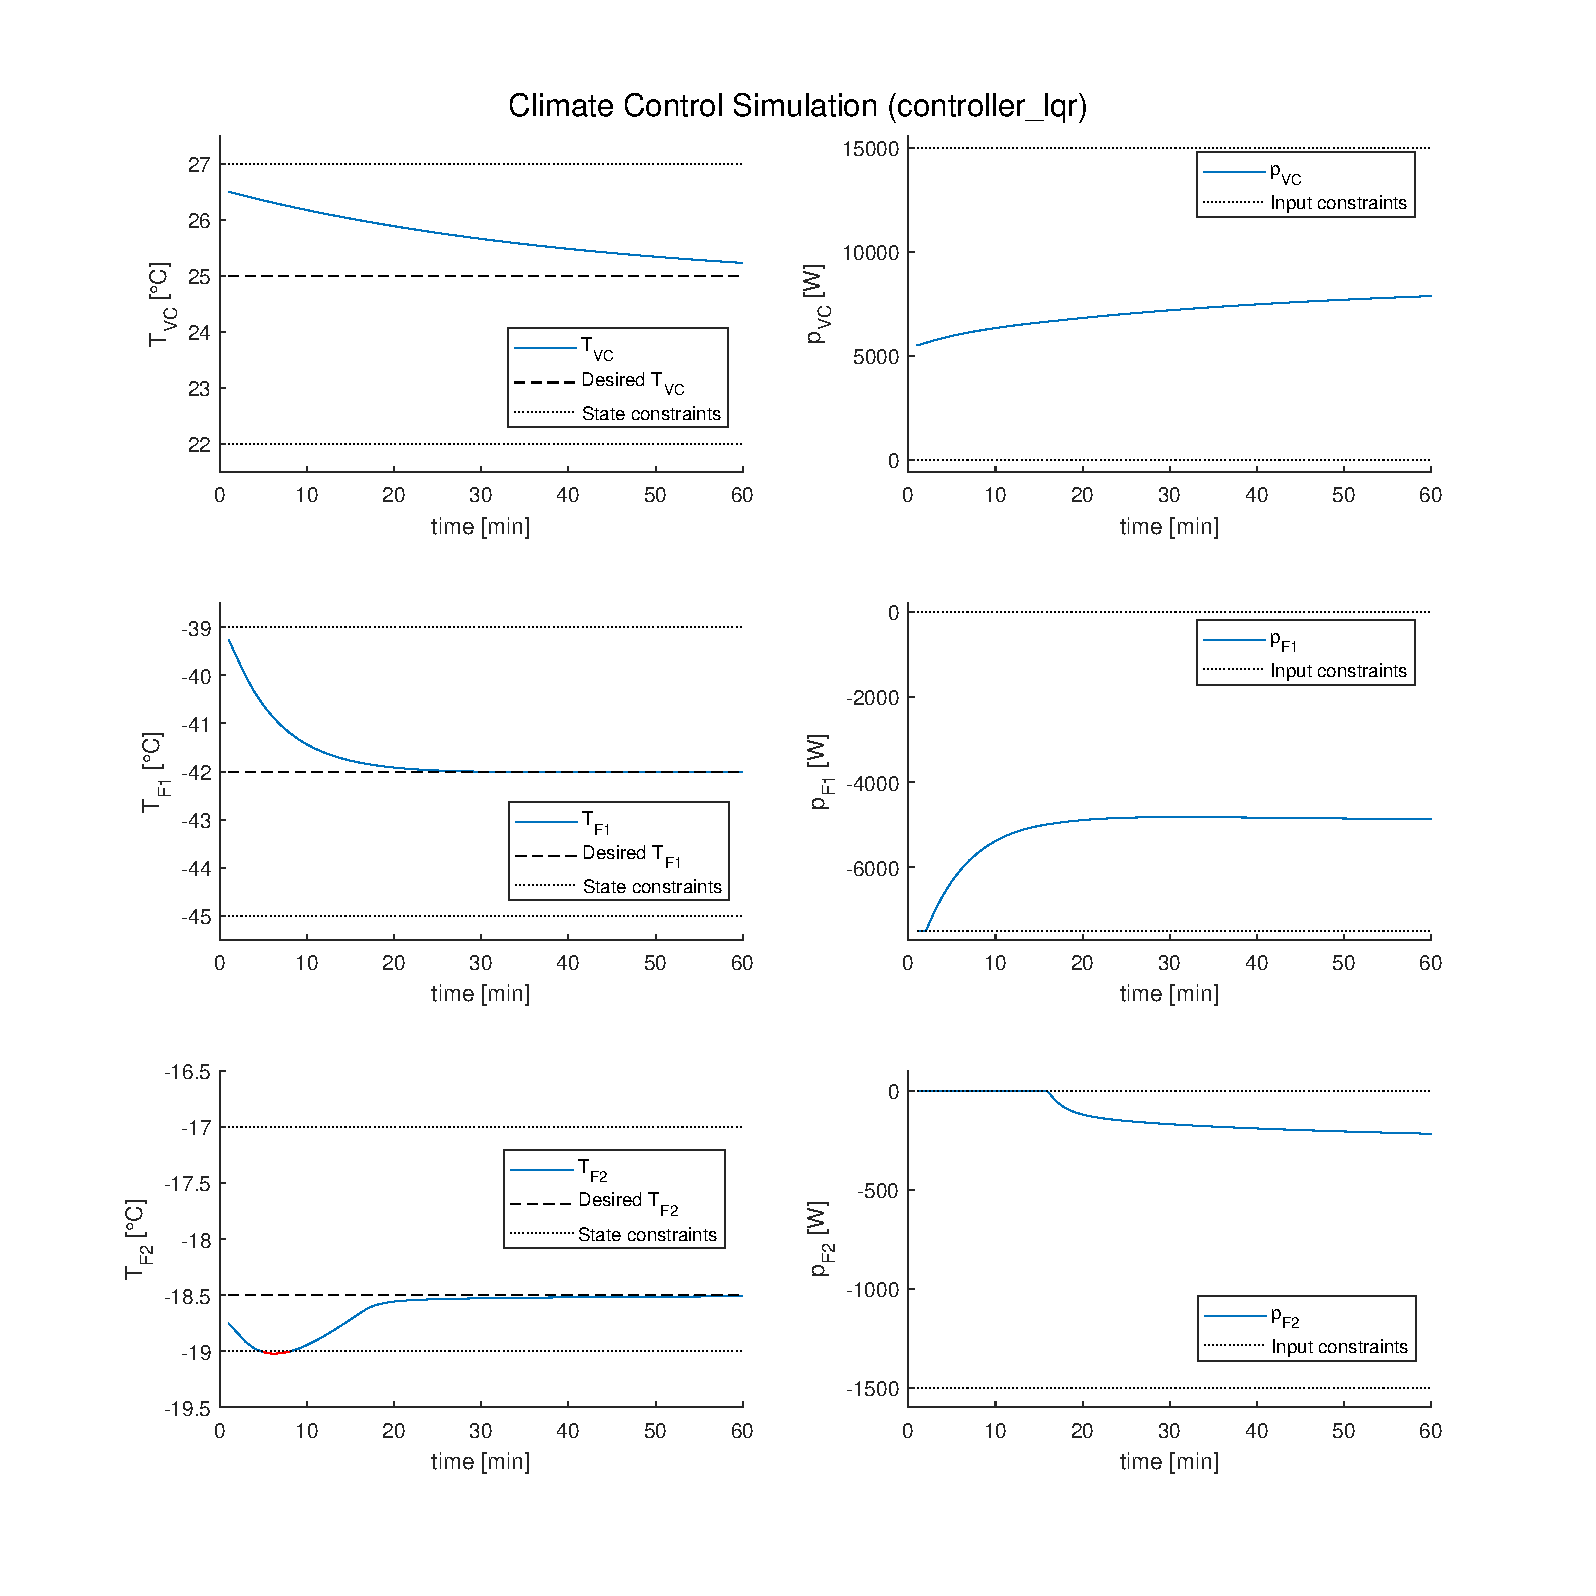
\includegraphics[scale = 0.58]{image/8.eps}
\caption{Simulation with initial condition 2 using LQR Controller}
\label{fig:4}
\end{figure}

Figure \ref{fig:4} shows the closed-loop simulation plot of the system under the LQR controller with the identity $R$ and the $Q$ found by the heuristic approach with the initial state $T(0) = T^{(2)}_{init} = T_{sp} + [1.5 \ 2.75 \ -0.25]^\top$. 

Comparing to the first initial state, the temperature in the room still converge slowly and the temperature in vaccination 1 will converge to the steady state fast. However, the cooling unit in vaccination 2 will not be working at first because we initialize the temperature in vaccination 2 below the steady state. When the heat is transported from the room and vaccination 1 to the vaccination 2, the cooling unit then starts to work. But it is already too late because the temperature in vaccination has already dropped below the minimum required temperature at around 7 minutes after simulation. 

This result shows that in most of the time, LQR controller has a good performance. However, LQR controller lacks the capability to implement the constraints, thus lacks the ability to make 'prediction' and acts ahead before it is too late. Besides, LQR controller is also sensitive to the initial state: wrong initial state may lead to a bad performance.

\newpage

%-------------------------------------------------------------------

\section{From LQR to model predictive controller}

\subsection{Task 9: LQR Feasible Set (3 pt.)}

In our control problem, we set $x(k) = \Delta T(k)$ and $u(k) = \Delta p(k)$, and also $x_{min} = \Delta T_{min}, x_{max} = \Delta T_{max}$ and $u_{min} = \Delta p_{min}, u_{max} = \Delta p_{max}$. Using \verb|system.LQRSet()| from the MPT toolbox we can easily calculate the LQR feasible set.

\begin{figure}[ht]
\centering
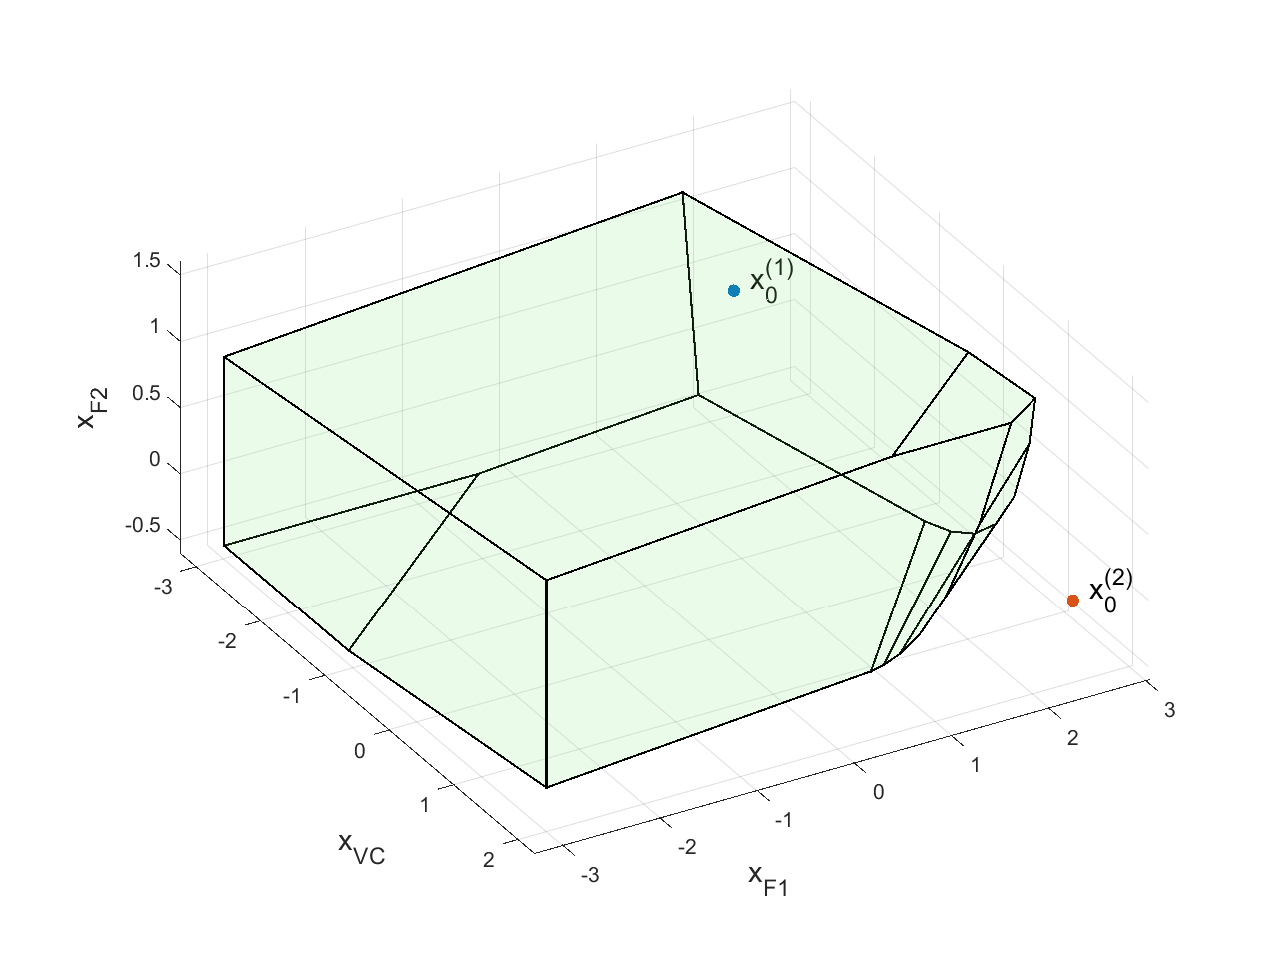
\includegraphics[scale = 0.6]{image/9.eps}
\caption{LQR feasible set}
\label{fig:5}
\end{figure}

Figure \ref{fig:5} shows the feasible set of the LQR controller (the initial state set which will not violate the state and input constraints all the time using LQR controller). From the plot, we also know that the first initial state lies in the feasible set while the second does not. We can conclude that any initial states in the feasible set will not cause any violation of the constraints using LQR controller.  

\subsection{Task 10: Infinite Horizon Cost under the LQR Control Law (1 pt.)}

Figure \ref{fig:6} shows the infinite horizon cost under the LQR control law. We can see from the scatter plot that the infinite horizon cost is mainly related to initial state of the building temperature. This is mainly because the building has only heating unit and a relatively large mass than the vaccinations, so the LQR controller will mainly deal with the difference from the building temperature and its steady state. 

If the building temperature is higher than the steady state, the heating unit will not function at first but wait the heat is removed from the building to the vaccinations and been cooled down using cooling units there. Thus, the infinite horizon cost will be lower. On the contrary, if the building temperature is already below the steady state, the heating unit will start to regulate the temperature immediately, which will naturally result in a larger input of the heating unit and lead to a larger infinite horizon cost. 

In comparison to the building temperature regulation, the vaccination temperatures are more easily regulated. On the one hand, the vaccination room will have a cooling unit and can decrease the temperature directly. On the other hand, the heat flow from the building to the vaccination can be easily increased using the heating unit in the building, if the temperature in the vaccination room is too low. 

\begin{figure}[ht]
\centering
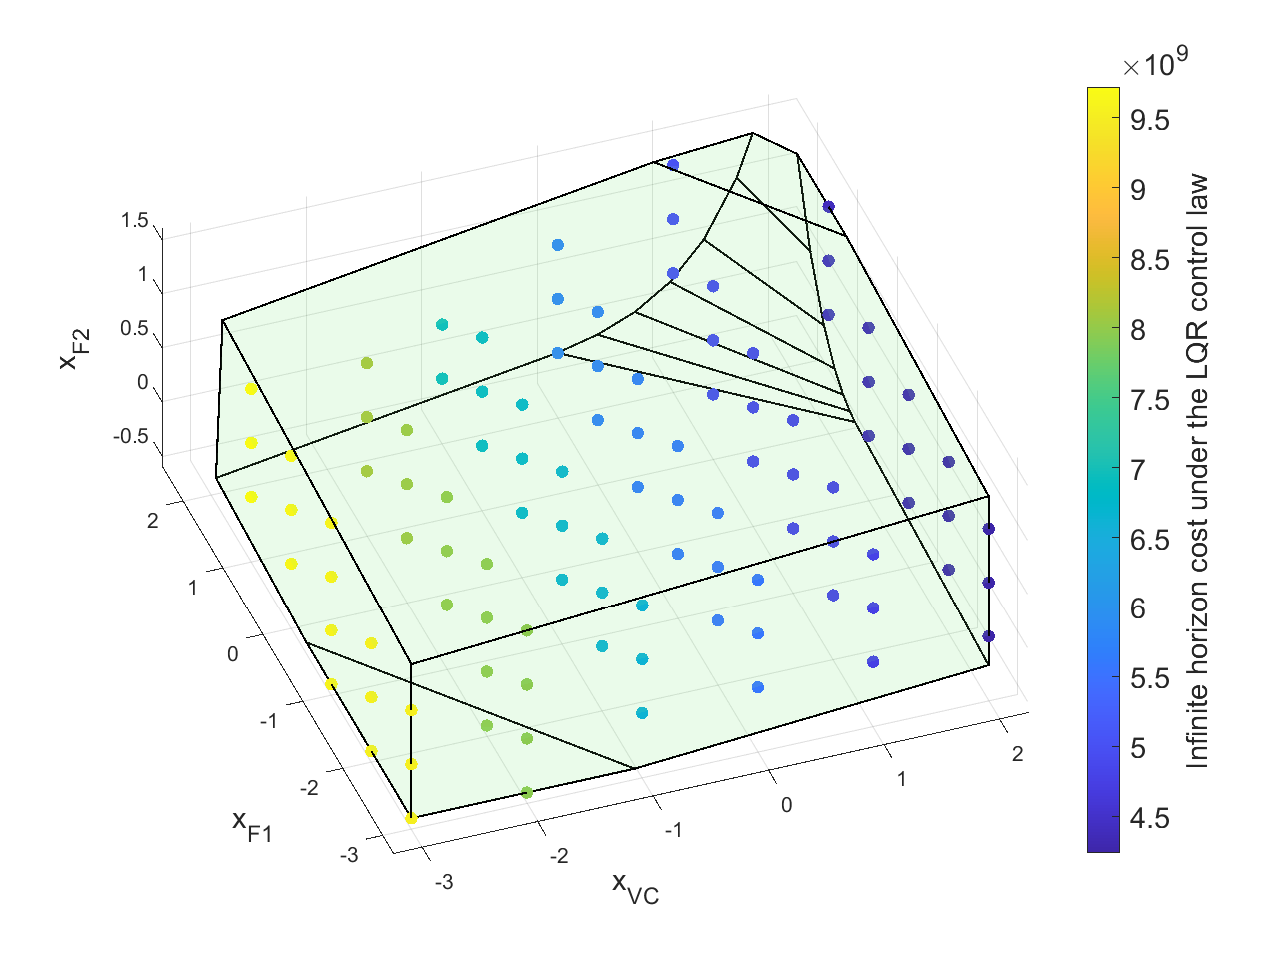
\includegraphics[scale = 0.6]{image/10.eps}
\caption{Infinite Horizon Cost under the LQR Control Law}
\label{fig:6}
\end{figure}

\subsection{Task 11: Model Predictive Controller 1 (5 pt.)}

Here we choose the terminal cost $I_f(x_N) = x_N^\top S x_N$, where $S = P_\infty$, which is the solution to the discrete-time algebraic Riccati equation. Figure \ref{fig:7} and figure \ref{fig:8} show the closed-loop simulation using model predictive controller 1 under the initial state $T^{(1)}_{init} = T_{sp} + [-2.25 \ 1.75 \ 0.75]^\top$ and $T^{(2)}_{init} = T_{sp} + [1.5 \ 2.75 \ -0.25]^\top$ respectively. 

Let's look at figure \ref{fig:7} first and compare the result with what we have got in figure \ref{fig:3}, which is the simulation using LQR controller. We have already calculated the feasible set of the LQR controller and know that the first initial state $T^{(1)}_{init} = T_{sp} + [-2.25 \ 1.75 \ 0.75]^\top$ lies in the feasible set of the LQR controller, which means that the following states and the LQR inputs will not violate the state and input constraints. In comparison, model predictive controller will achieve the same result, because the prediction it makes at every time-step will not violate the state and input constraints either. As a result, the model predictive controller acts the same as the LQR controller. 

Then how about figure \ref{fig:8}? As observed above, the LQR controller will violate the state constraints, specifically, the state constraint of $T_{F2}$, because the initial state $T^{(2)}_{init} = T_{sp} + [1.5 \ 2.75 \ -0.25]^\top$ is not in the feasible set of the LQR controller. However, the model predictive controller does a much better job and will not violate any constraints. The model predictive controller implemented the constraints in the prediction, so the cooling unit in vaccination 2 will start earlier than LQR controller. And we an see that the temperature in vaccination 2 will not drop below the minimum allowed temperature. 

To conclude, the model predictive controller will achieve better performance because of its implementation of the constraints and the capability to predict and act beforehand. 

\begin{figure}[ht]
\centering
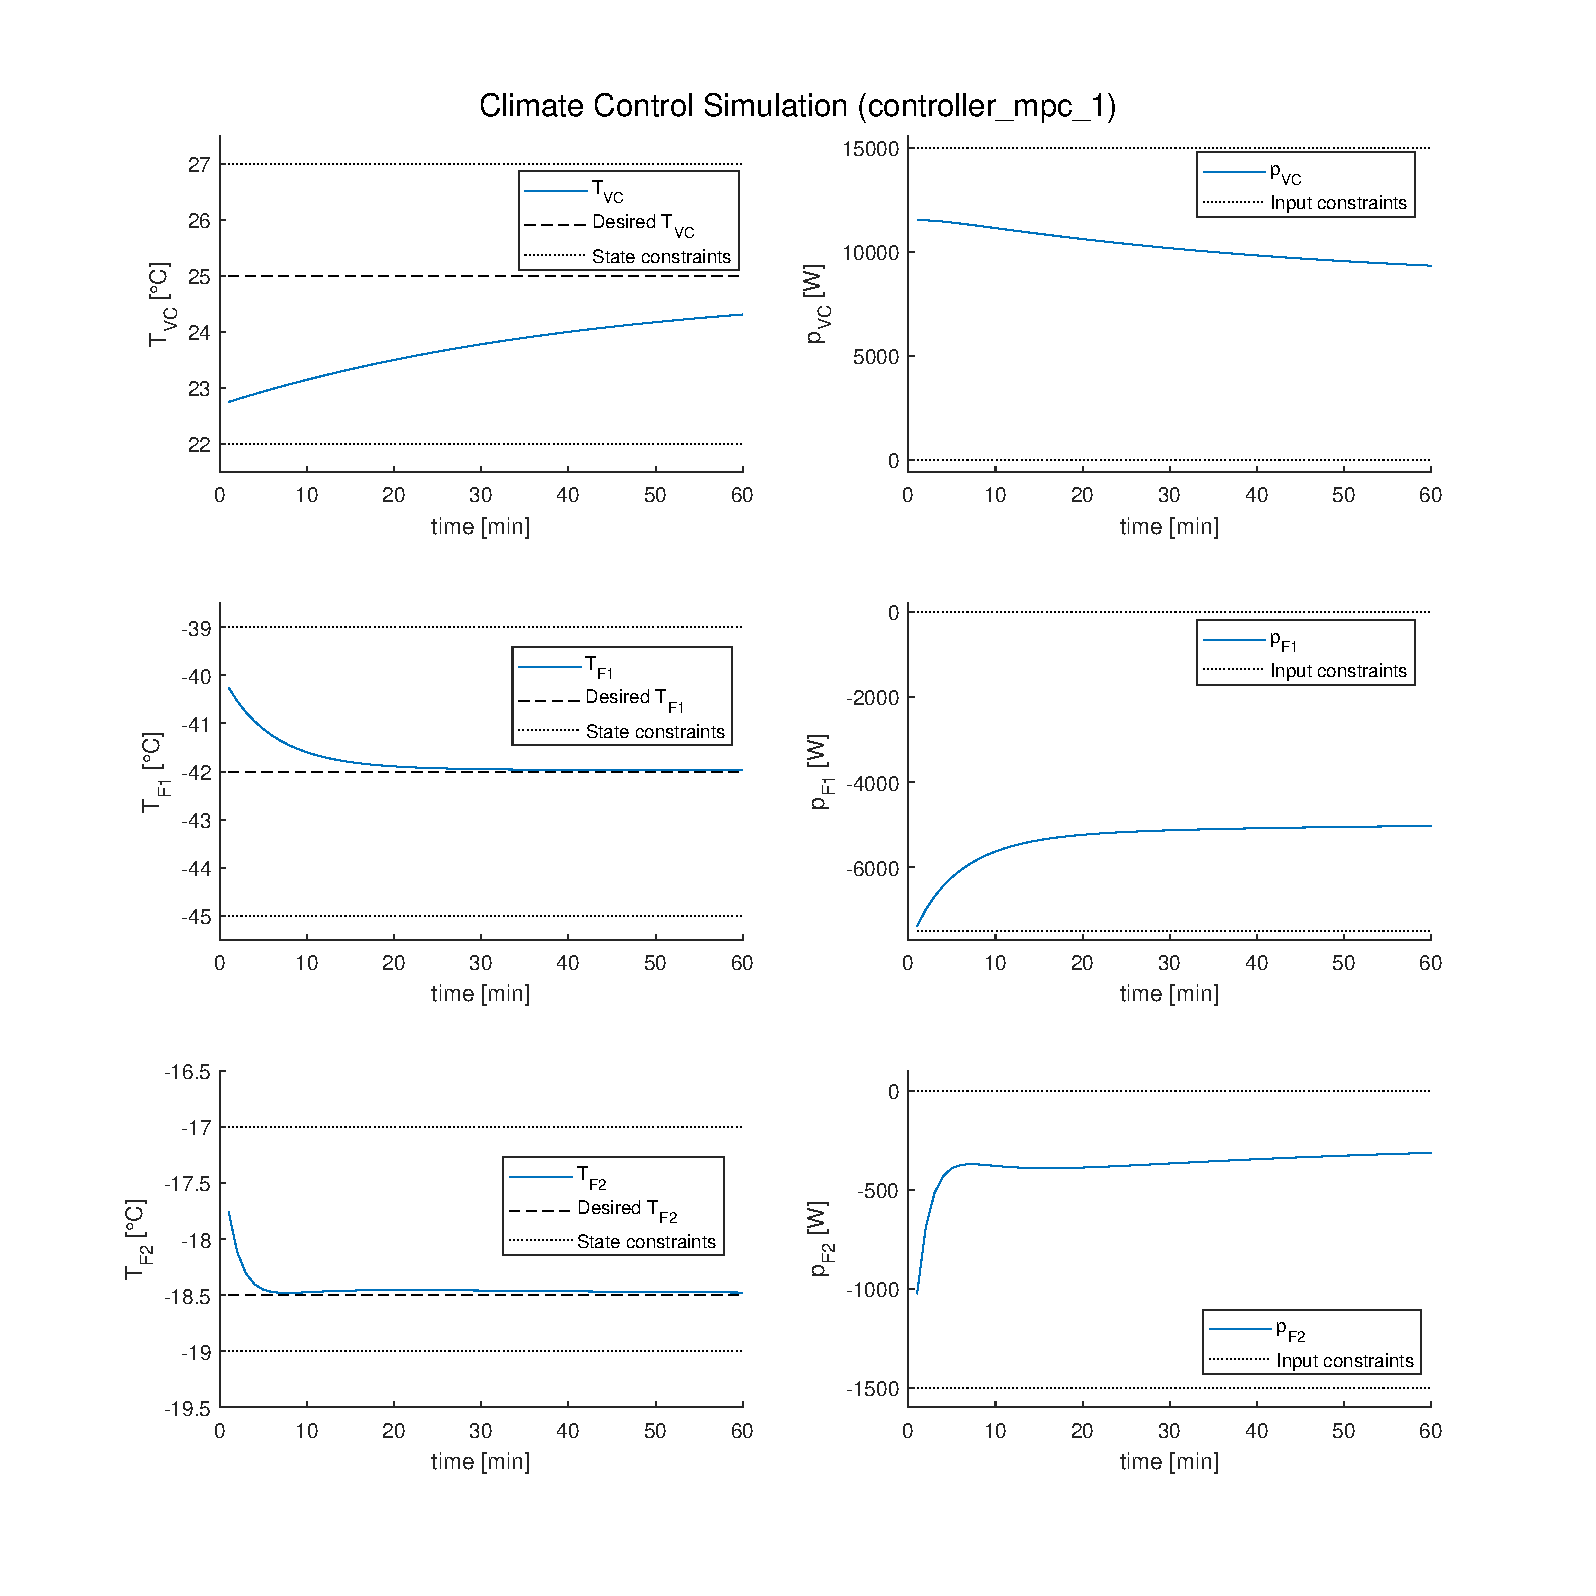
\includegraphics[scale = 0.58]{image/11-1.eps}
\caption{Simulation with initial condition 1 using Model Predictive Controller 1}
\label{fig:7}
\end{figure}

\newpage

\begin{figure}[ht]
\centering
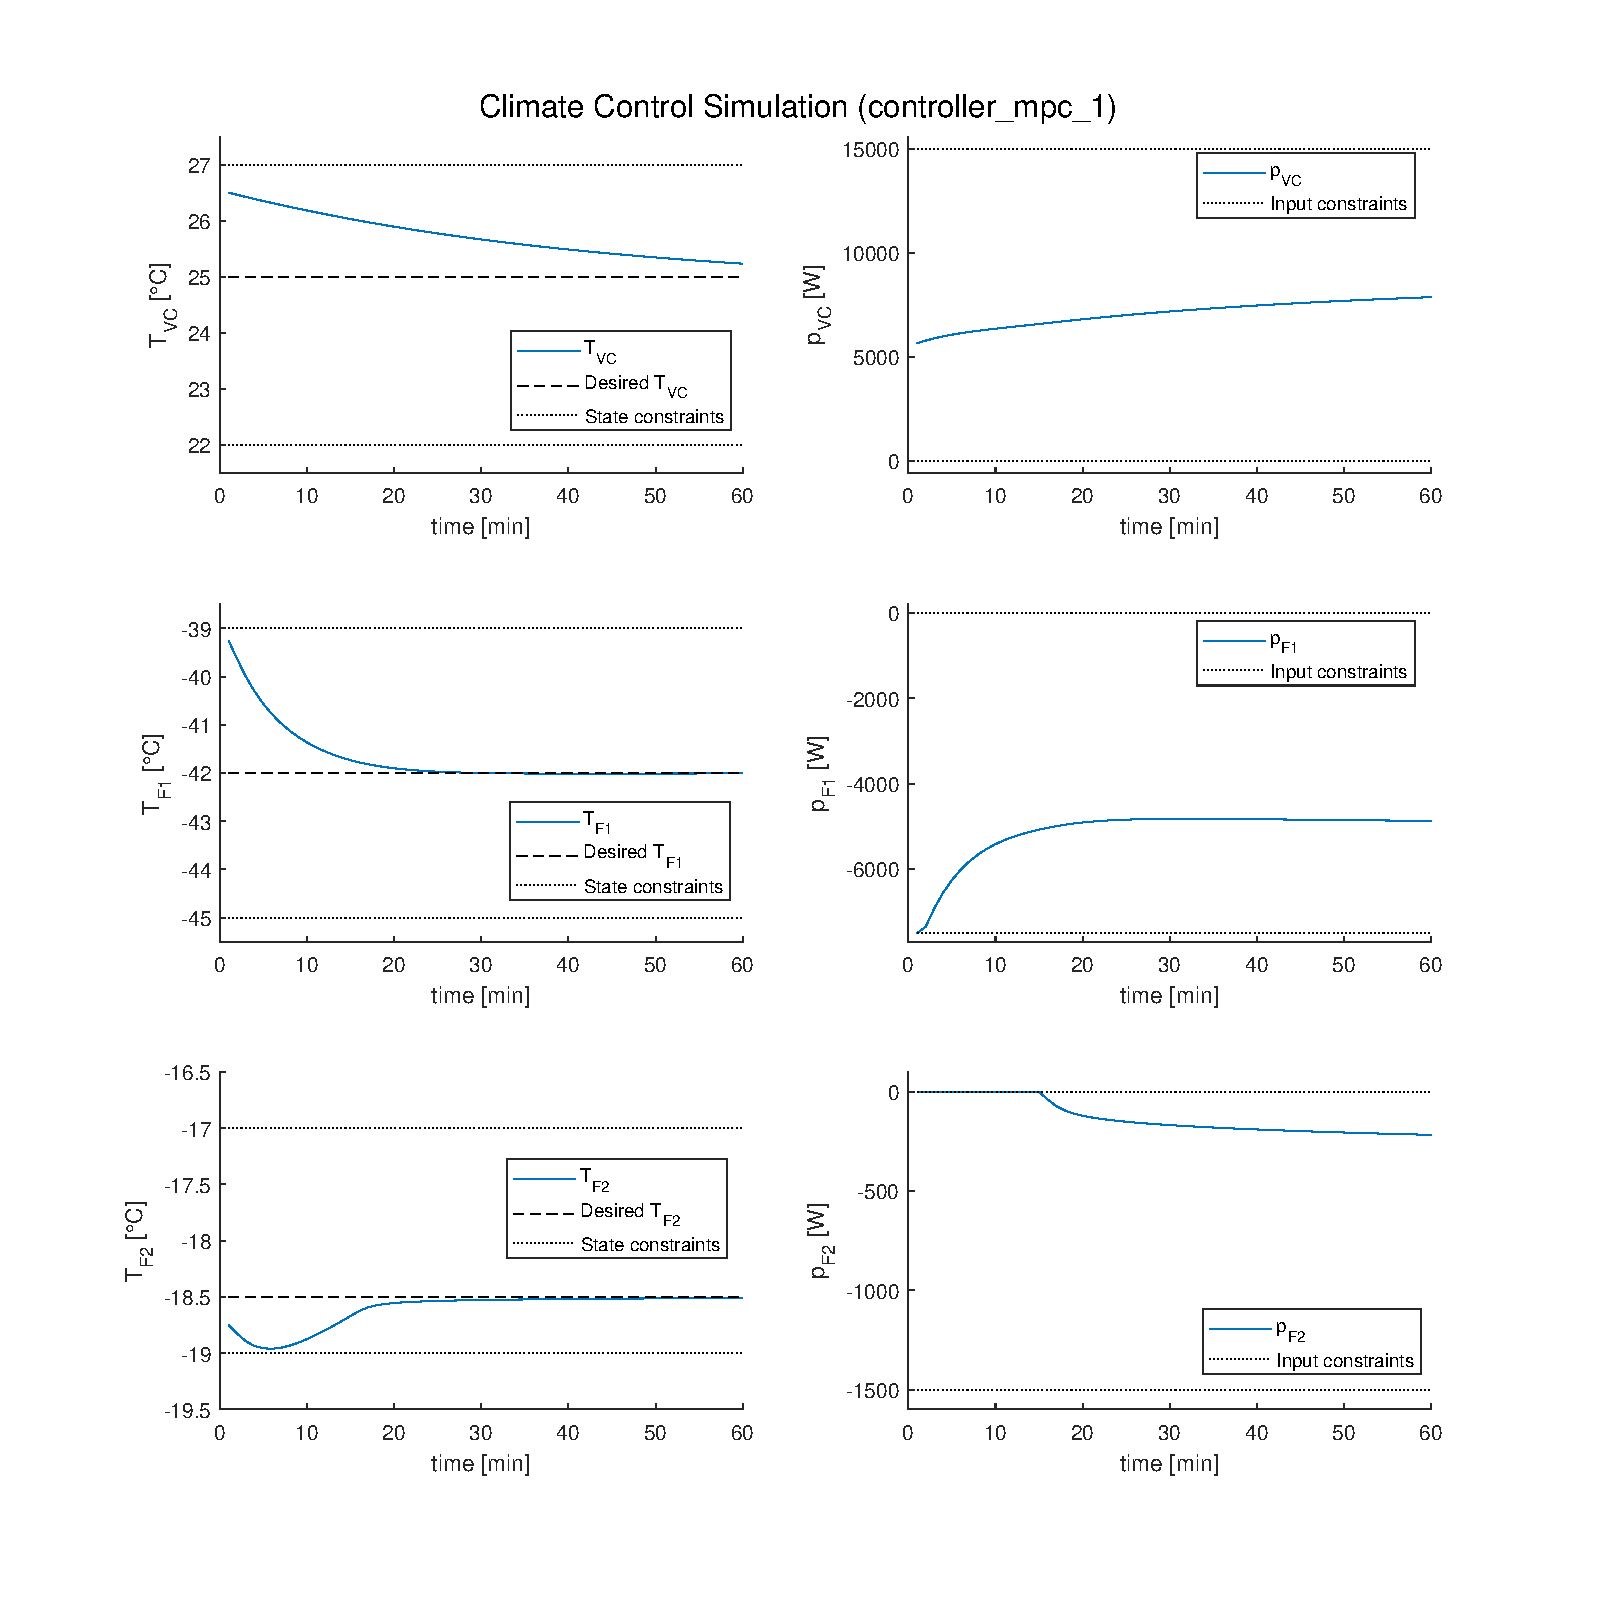
\includegraphics[scale = 0.58]{image/11-2.eps}
\caption{Simulation with initial condition 2 using Model Predictive Controller 1}
\label{fig:8}
\end{figure}

\newpage

%---------------------------------------------------------------------------------

\section{MPC with theoretical closed-loop guarantees}

\subsection{Task 12: Asymptotic Stability with Zero Terminal Constraint (2 pt.)}

As we see from the structure of the MPC problem, the terminal cost $l_f(x_N) = 0$ and we add a terminal state constraint $x_{30} = 0$. The origin is an equilibrium point because the optimal input is 0 and the state will stay at the origin forever. We will prove the asymptotic stability of the origin recursively. 

First, we already know that $x(0)$ is feasible for the MPC problem, which is given. And we assume that the feasibility of $x(k)$ and let $\{u^*_0, u^*_1, \cdots, u^*_{N-1}\}$ be the optimal control sequence computed at $x(k)$ and let $\{x(k), x_1^*, \cdots, x_N^*\}$ be the corresponding state trajectory. We will apply $u(k) = u^*_0$ and let the system evolve to $x(k+1) = Ax(k)+Bu(k)$. We can observe that at time k+1, $x(k+1) = x_1^*$. And we propose a shifted control sequence $\Tilde{U} = \{u^*_1, u^*_2, \cdots, u^*_{N-1}, 0\}$. Because $x^*_N = 0$ and $Ax^*_N+B\cdot 0 =0$, the shifted control sequence is feasible (but not necessarily optimal). 

Then we propose a Lyapunov function $V(x(k)) = J^*(x(k))$, which is the optimal cost at time k. We notice that $J^*(0) = 0$ and $J^*(x(k)) = \sum_{i = 0}^{30-1}l(x_i^*, u_i^*)>0$ for $x(k) \neq 0$. And by applying the shifted control sequence, we also have
\begin{equation*}
    \begin{split}
        J^*(x(k+1)) & \le \Tilde{J}(x(k+1)) = \sum_{i = 0}^{30-1}l(x_i, \Tilde{u}_i) \\
                    & = \sum_{i = 1}^{30-1}l(x_i^*, u_i^*) = \sum_{i = 1}^{30-1}l(x_i^*, u_i^*) + l(x(k), u_0^*) - l(x(k), u_0^*) \\
                    & = J^*(x(k)) - l(x(k), u_0^*) < J^*(x(k))
    \end{split}
\end{equation*}

Thus we have $V(x(k+1))- V(x(k)) \le \alpha(x(k))$ for $x(k) \neq 0$, where $\alpha$ is positive definite. Then using Lyapunov stability theorem we can confirm that the origin is an asymptotically stable equilibrium point for the resulting closed-loop system. 

\subsection{Task 13: Model Predictive Controller 2 (3 pt.)}

Figure \ref{fig:9} and figure \ref{fig:10} show the closed-loop simulation using model predictive controller 2 under the initial state $T^{(1)}_{init} = T_{sp} + [-2.25 \ 1.75 \ 0.75]^\top$ and $T^{(2)}_{init} = T_{sp} + [1.5 \ 2.75 \ -0.25]^\top$. Here we only add a terminal state constraint $x^*_N = 0$ to our MPC controller, which will force the prediction ending at the origin at each time step. 

For the first initial state, the model predictive controller with terminal state constraint will force the building temperature to converge faster than the model predictive controller without terminal state constraint, while adding trivial influence on the convergence of the temperatures in vaccination 1 and 2. 

However, for the second initial state, we noticed that the temperature in vaccination 2 will stay at the minimum allowed temperature for about 10 minutes. Even if all the temperatures will not violate the constraints, the controller performs not so well. This is mainly because the time horizon (30 minutes by default) is relatively long, the cooling unit in vaccination 2 will not take any action (to reduce the input cost) if the other units (heating unit in the building and the cooling unit in vaccination 1) are able to drive the system to the origin at the end of the prediction while not violating the constraints. 

\newpage

\begin{figure}[ht]
\centering
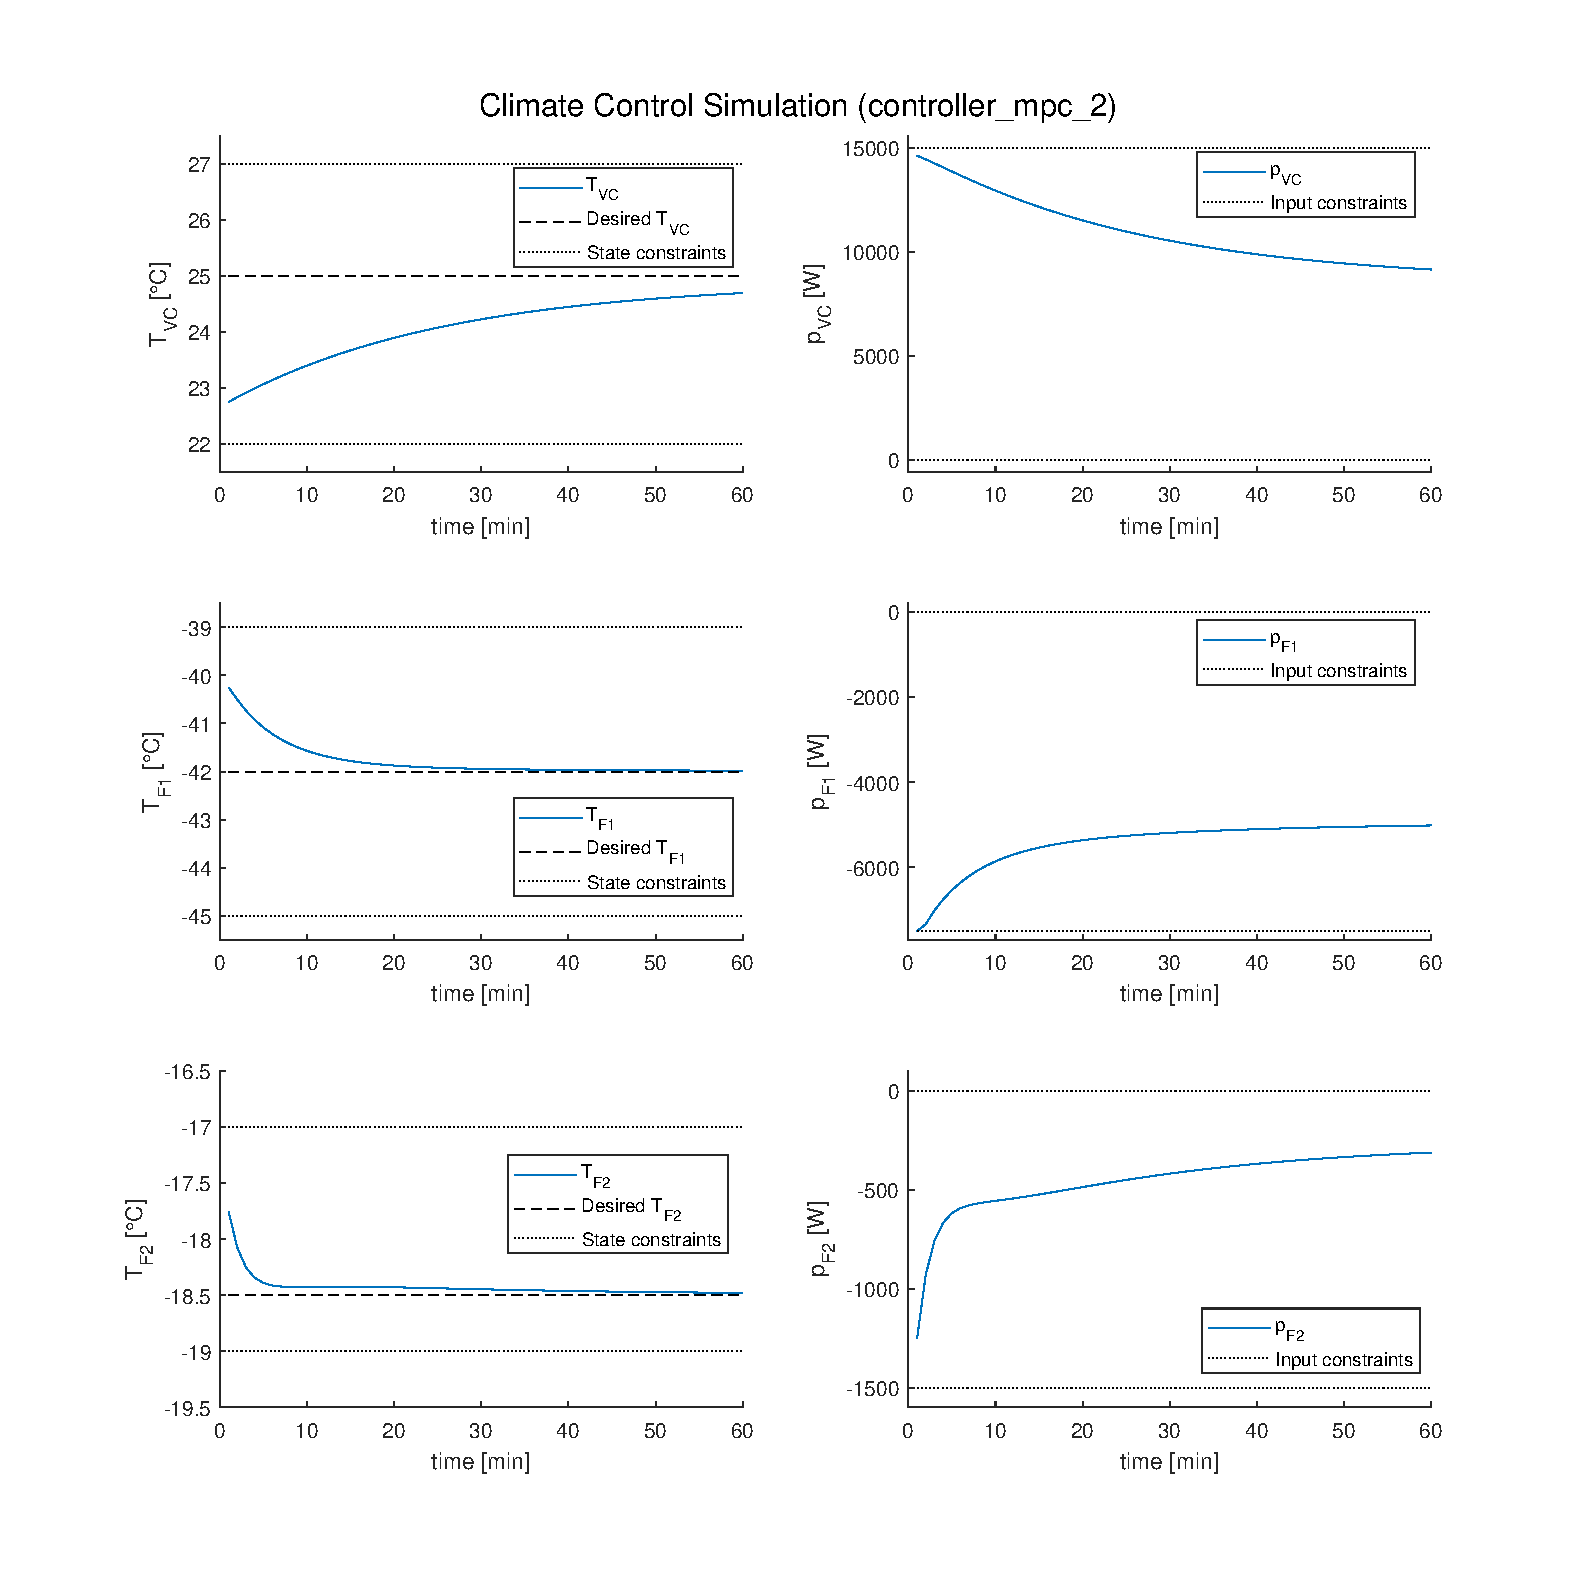
\includegraphics[scale = 0.58]{image/13-1.eps}
\caption{Simulation with initial condition 1 using Model Predictive Controller 2}
\label{fig:9}
\end{figure}

\newpage

\begin{figure}[ht]
\centering
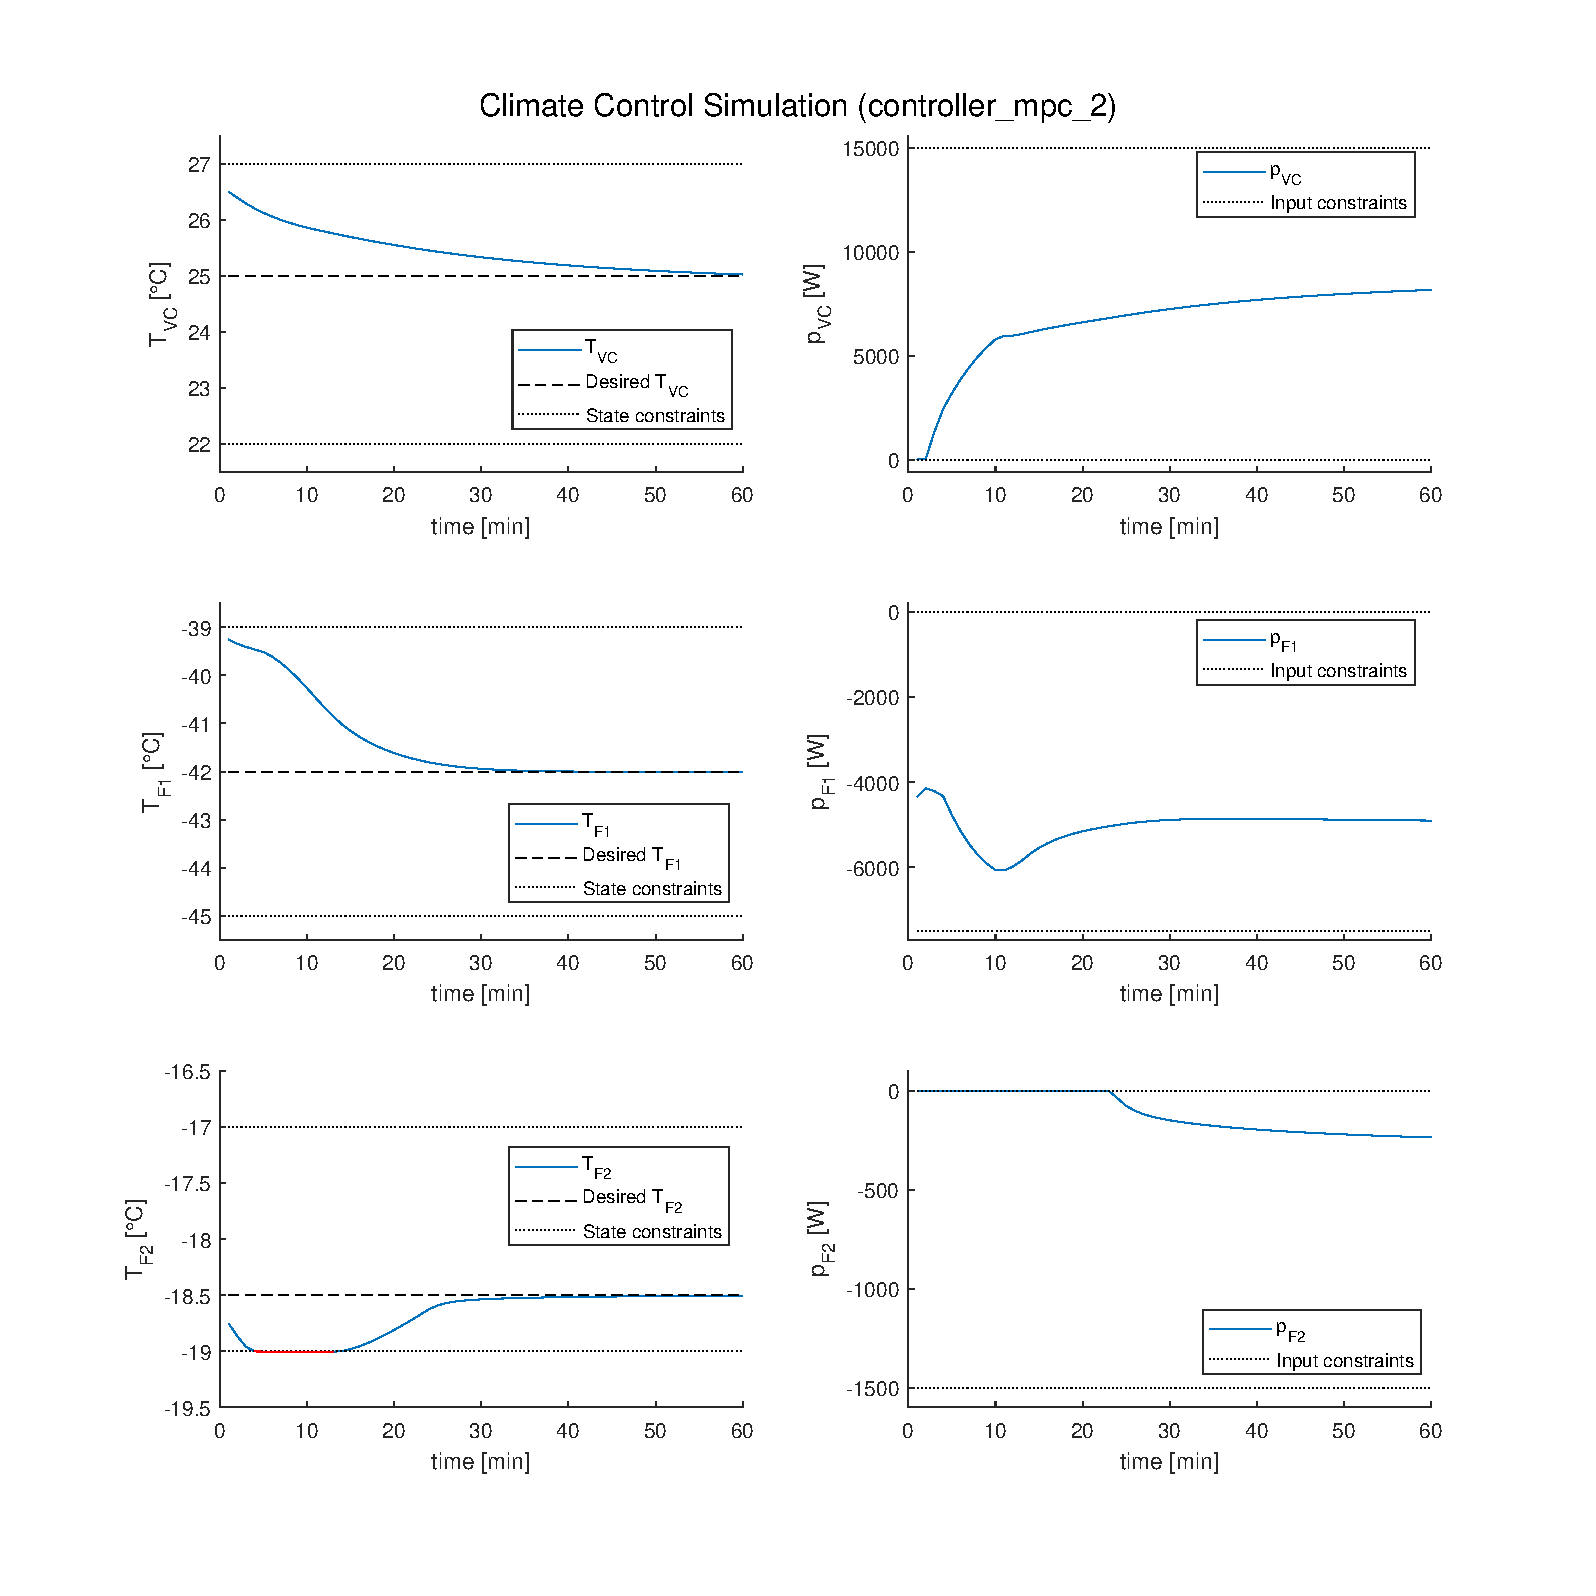
\includegraphics[scale = 0.58]{image/13-2.eps}
\caption{Simulation with initial condition 2 using Model Predictive Controller 2}
\label{fig:10}
\end{figure}

\subsection{Task 14: Model Predictive Controller 3 (5 pt.)}

Here we choose the terminal cost $l_f(x) = P_\infty$, which is the solution to the discrete-time algebraic Riccati equation. By construction the terminal cost is a continuous Lyapunov function in the terminal set $X_{LQR}$ and satisfies
\begin{equation*}
    \begin{split}
        x^\top_{k+1} P_\infty x_{k+1}-x^\top_k P x_k &= x^\top_k(-P_\infty + A^\top P_\infty A + F_\infty^\top B^\top P_\infty A - F^\top_\infty R F_\infty)x_k \\
        &= -x^\top_k(Q + F^\top_\infty R F_\infty)x_k < 0
    \end{split}
\end{equation*}

Thus, the origin is an asymptotically stable equilibrium. 

Figure \ref{fig:11} and figure \ref{fig:12} show the closed-loop simulation using model predictive controller 3 under the initial state $T^{(1)}_{init}$ and $T^{(2)}_{init}$ respectively. 

\newpage

\begin{figure}[ht]
\centering
\includegraphics[scale = 0.58]{image/14-1.eps}
\caption{Simulation with initial condition 1 using Model Predictive Controller 3}
\label{fig:11}
\end{figure}

\newpage

\begin{figure}[ht]
\centering
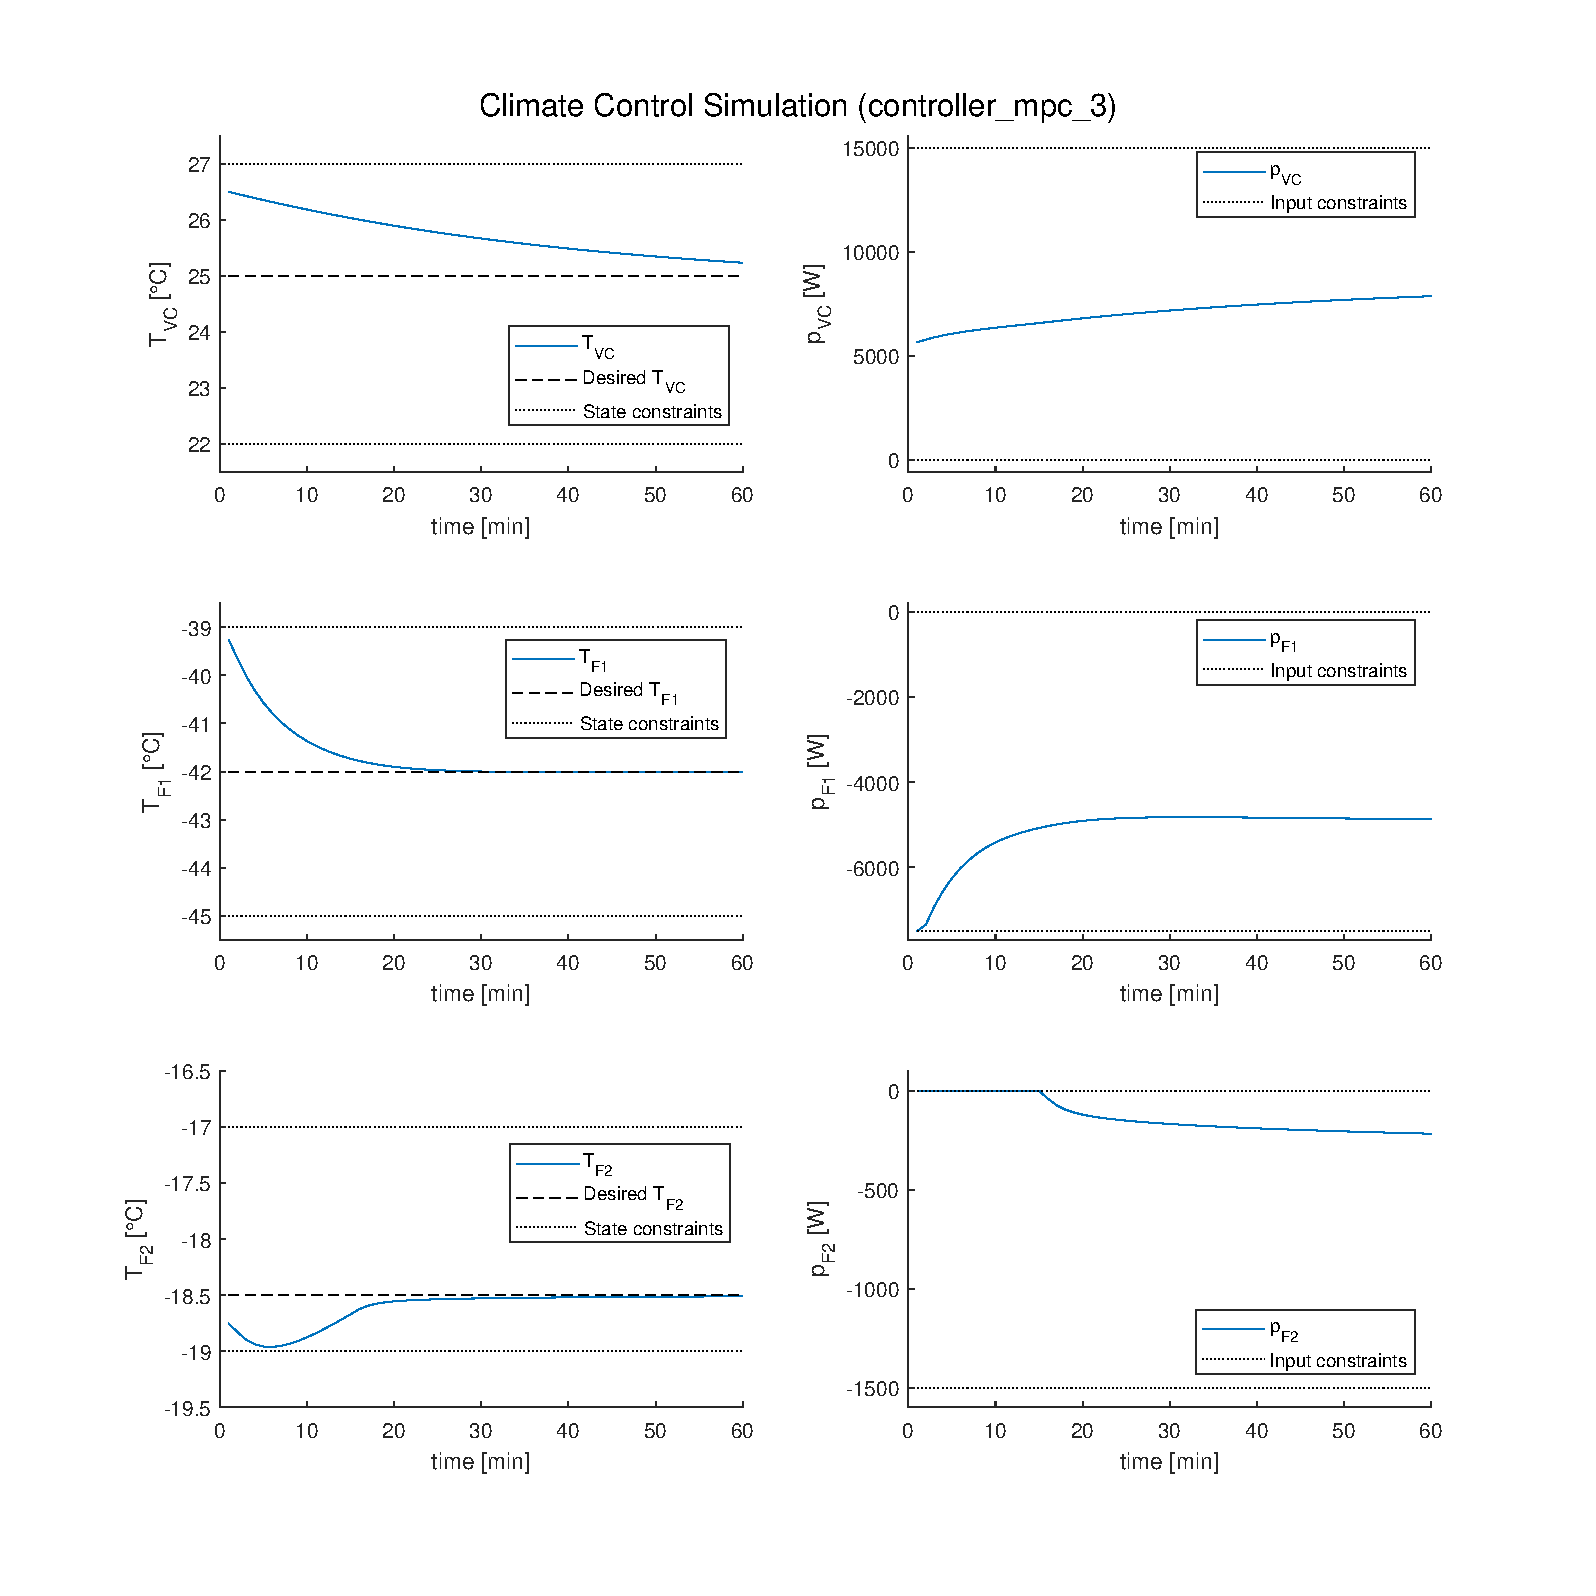
\includegraphics[scale = 0.58]{image/14-2.eps}
\caption{Simulation with initial condition 2 using Model Predictive Controller 3}
\label{fig:12}
\end{figure}

\newpage

\subsection{Task 15: Discussion on the Three MPC Controllers (2 pt.)}

Figure \ref{fig:13} and figure \ref{fig:14} show the closed-loop simulations using model predictive controller 1-3 under the initial state $T^{(1)}_{init}$ and $T^{(2)}_{init}$ respectively. For the states (on the left side), lines in \textcolor{ORANGE}{orange} correspond to MPC controller 1 and 3, and lines in \textcolor{GREEN}{green} correspond to MPC controller 2. For the inputs (on the right side), lines in \textcolor{RED}{red} correspond to MPC controller 1 and 3, and lines in \textcolor{PURPLE}{purple} correspond to MPC controller 2. 

The optimization costs for the MPC controllers under the initial state $T^{(1)}_{init}$ are
\begin{equation*}
    J_{MPC1}(T^{(1)}_{init}) = 8.563\times10^9
\end{equation*}
\begin{equation*}
    J_{MPC2}(T^{(1)}_{init}) = 9.483\times10^9
\end{equation*}
\begin{equation*}
    J_{MPC3}(T^{(1)}_{init}) = 8.563\times10^9
\end{equation*}

The optimization costs for the MPC controllers under the initial state $T^{(2)}_{init}$ are
\begin{equation*}
    J_{MPC1}(T^{(2)}_{init}) = 4.817\times10^9
\end{equation*}
\begin{equation*}
    J_{MPC2}(T^{(2)}_{init}) = 4.584\times10^9
\end{equation*}
\begin{equation*}
    J_{MPC3}(T^{(2)}_{init}) = 4.817\times10^9
\end{equation*}

Firstly, we noticed that MPC controller 1 and 3 will achieve the same simulation results for both initial states in terms of numerical accuracy. The only difference between MPC controller 1 and 3 is the terminal state constraint $x_{30}\in X_{LQR}$. The results shows that the terminal state constraint is always loose, which means that in the predictive trajectory, the terminal state will always lie in the LQR feasible set. By comparing the optimization costs, we will have the same conclusion.

Secondly, let's talk about the performance of the MPC controller 2. MPC controller 2 removes the terminal cost and change the terminal state constraint to a much stronger one, zero terminal constraint $x_{30}=0$. For the fist initial state, MPC controller 2 will drive the building temperature to converge faster than the other two controllers but use more resource of the heating unit. This is mainly because the terminal state constraint in MPC 2 is more difficult to fulfill, and the optimization cost also confirms this conclusion. However, for the second initial state, MPC controller 2 doesn't have a satisfactory performance even if it has a better optimization cost than the other two controllers. MPC controller 2 reduces the input cost but increases the state cost, and it also sacrifices the state convergence to let the temperature in vaccination 2 stays around the minimum allowed temperature for about 10 minutes. 

To conclude, it is sometimes dangerous to achieve the stability and feasibility of the MPC controller by forcing the terminal state to be the origin, because zero terminal constraint reduces the size of the feasible set. A wiser way is to add a valid terminal set, which is invariant under some control law. 

\newpage

\begin{figure}[ht]
\centering
\includegraphics[scale = 0.58]{image/15-1.eps}
\caption{Comparison between MPC controller 1-3 with initial condition 1}
\label{fig:13}
\end{figure}

\newpage

\begin{figure}[ht]
\centering
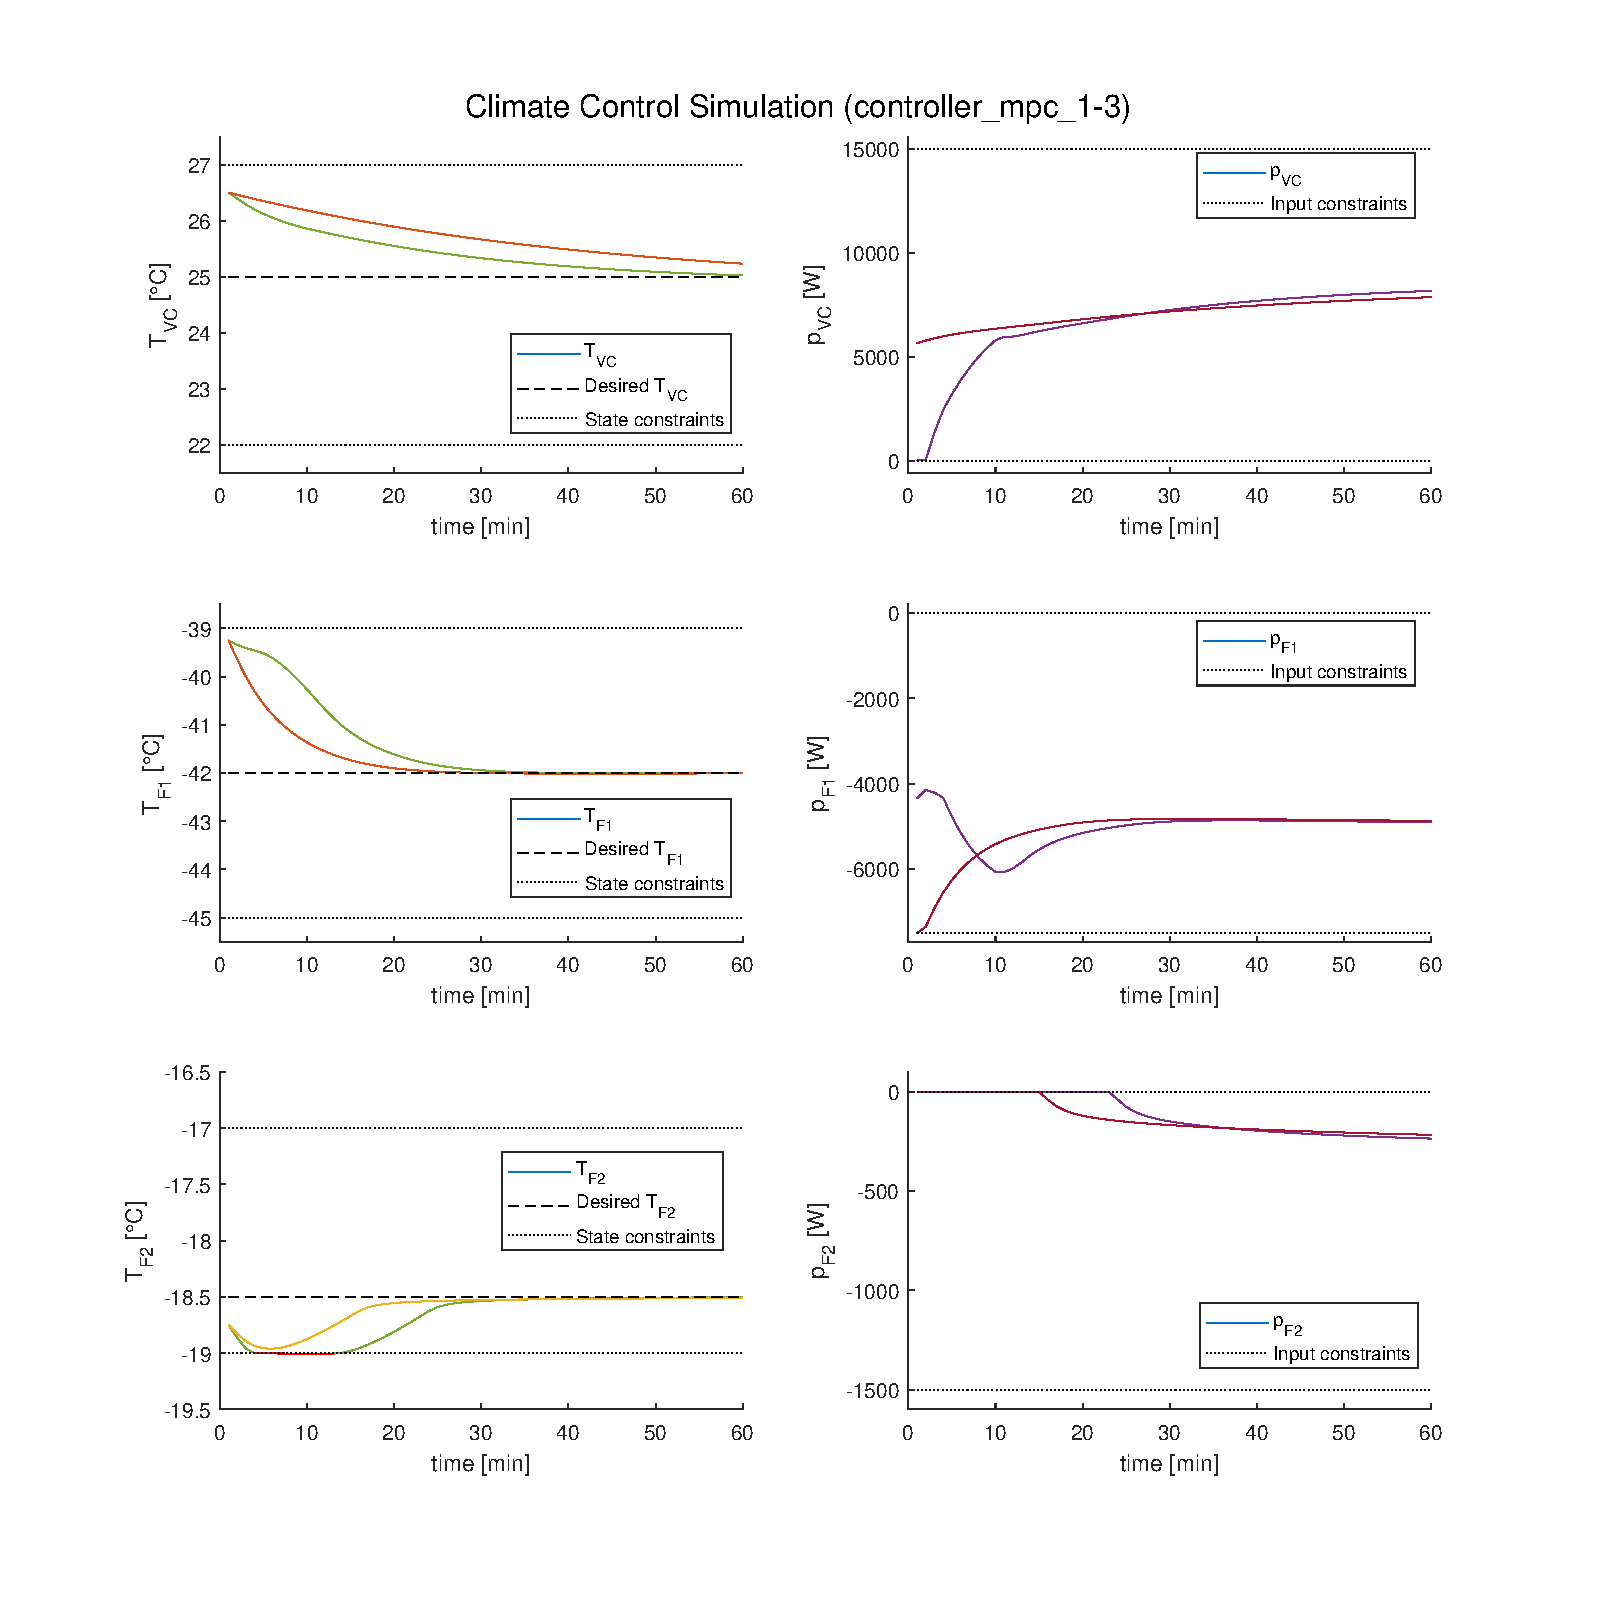
\includegraphics[scale = 0.58]{image/15-2.eps}
\caption{Comparison between MPC controller 1-3 with initial condition 2}
\label{fig:14}
\end{figure}

\subsection{Task 16: The Intersection of Different Terminal Sets (4 pt.)}

The intersection $\chi_f\cap X_{LQR}$ is also an invariant set under the LQR controller $u(k) = F_\infty x_{LQR}(k)$. For any $x(k)\in \chi_f$, we have $x(k+1) = Ax(k)+BF_\infty x(k) \in \chi_f$ ($\chi_f$ is an invariant set). For any $x(k)\in X_{LQR}$, we have $x(k+1) = Ax(k)+BF_\infty x(k) \in X_{LQR}$ ($X_{LQR}$ is an invariant set). Thus, we will have for any $x(k)\in \chi_f\cap X_{LQR}$, $x(k+1) = Ax(k)+BF_\infty x(k) \in \chi_f\cap X_{LQR}$. So the intersection $\chi_f\cap X_{LQR}$ is also an invariant set under the LQR controller $u(k) = F_\infty x_{LQR}(k)$.

The MPC problem with the terminal set $\chi_f\cap X_{LQR}$ also yields an asymptotically stable MPC controller. Here we choose the terminal cost $l_f(x) = P_\infty$, which is the solution to the discrete-time algebraic Riccati equation. As proved before, the terminal cost is a continuous Lyapunov function in the terminal set $\chi_f\cap X_{LQR}$ by construction,  and satisfies
\begin{equation*}
    \begin{split}
        x^\top_{k+1} P_\infty x_{k+1}-x^\top_k P x_k &= x^\top_k(-P_\infty + A^\top P_\infty A + F_\infty^\top B^\top P_\infty A - F^\top_\infty R F_\infty)x_k \\
        &= -x^\top_k(Q + F^\top_\infty R F_\infty)x_k < 0
    \end{split}
\end{equation*}

Thus, the MPC problem with the terminal set $\chi_f\cap X_{LQR}$ also yields an asymptotically stable MPC controller. 

\newpage

%----------------------------------------------------------------------------

\section{Soft constraints}

\subsection{Task 17: Simulation of Scenario 2 Using MPC Controller 3 (2 pt.)}

Figure \ref{fig:15} shows the simulation plot of scenario 2 with initial condition 1 using MPC controller 3. We notice that start from 42 minutes after the start of simulation, the MPC controller becomes infeasible. The heating unit stops working and the cooling units work in full power, which results in the huge drop of the temperatures in the building and the vaccinations. In scenario 1, we assume that the disturbances are constant, but obviously it is not always the case, so in scenario 2, the disturbances vary with time. As a result, the MPC controller designed for the stationary disturbance doesn't deliver a satisfactory output. 

\begin{figure}[ht]
\centering
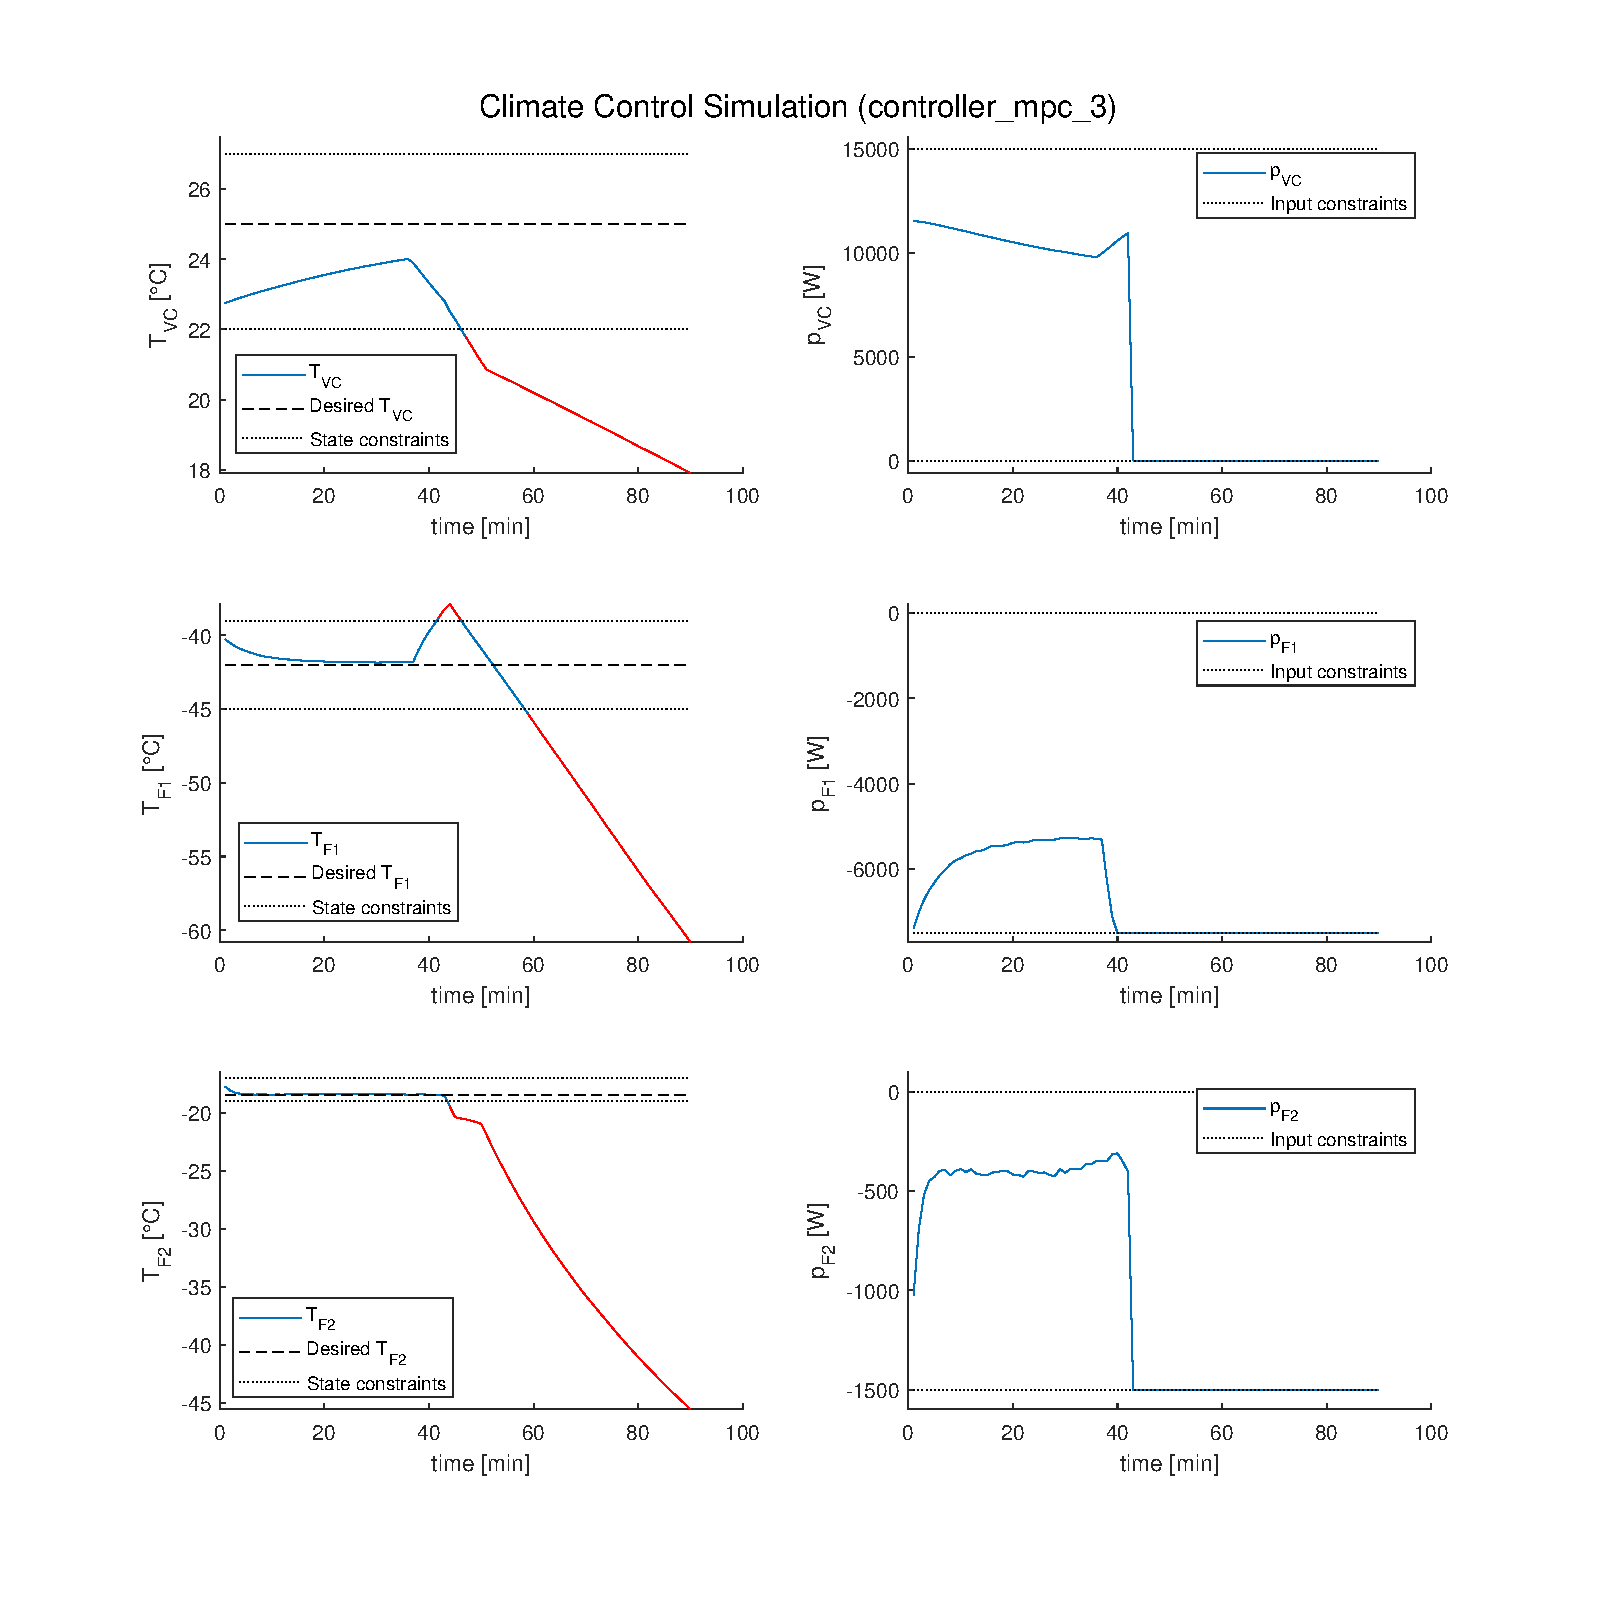
\includegraphics[scale = 0.58]{image/17.eps}
\caption{Simulation of Scenario 2 with initial condition 1 Using MPC Controller 3}
\label{fig:15}
\end{figure}

\subsection{Task 18: Soft-constrained MPC Controller (4 pt.)}

Figure \ref{fig:16} shows the simulation plot of scenario 2 using soft-constrained MPC controller. We notice that even if the initial condition at some time step is out of the feasible range, the soft-constrained MPC controller can still produce a reasonable input that drives the system to the steady state. Here we introduce slack variables $\epsilon_i$ to relax the state constraints and use the linear penalty $I_\epsilon(\epsilon) = v \cdot ||\epsilon||_1$ in the cost function. By choosing different $v$ values, we find out that the soft-constrained MPC controller will result in the same control input. The optimizer will choose $\epsilon_i$ such that the relaxed state constraints will not be violated, and it will keep the norm of $\epsilon_i$ as small as possible to reduce the optimization objective. No matter what $v$ we choose, the optimizer will take the same $\epsilon_i$ and also the input will be the same. 

\begin{figure}[ht]
\centering
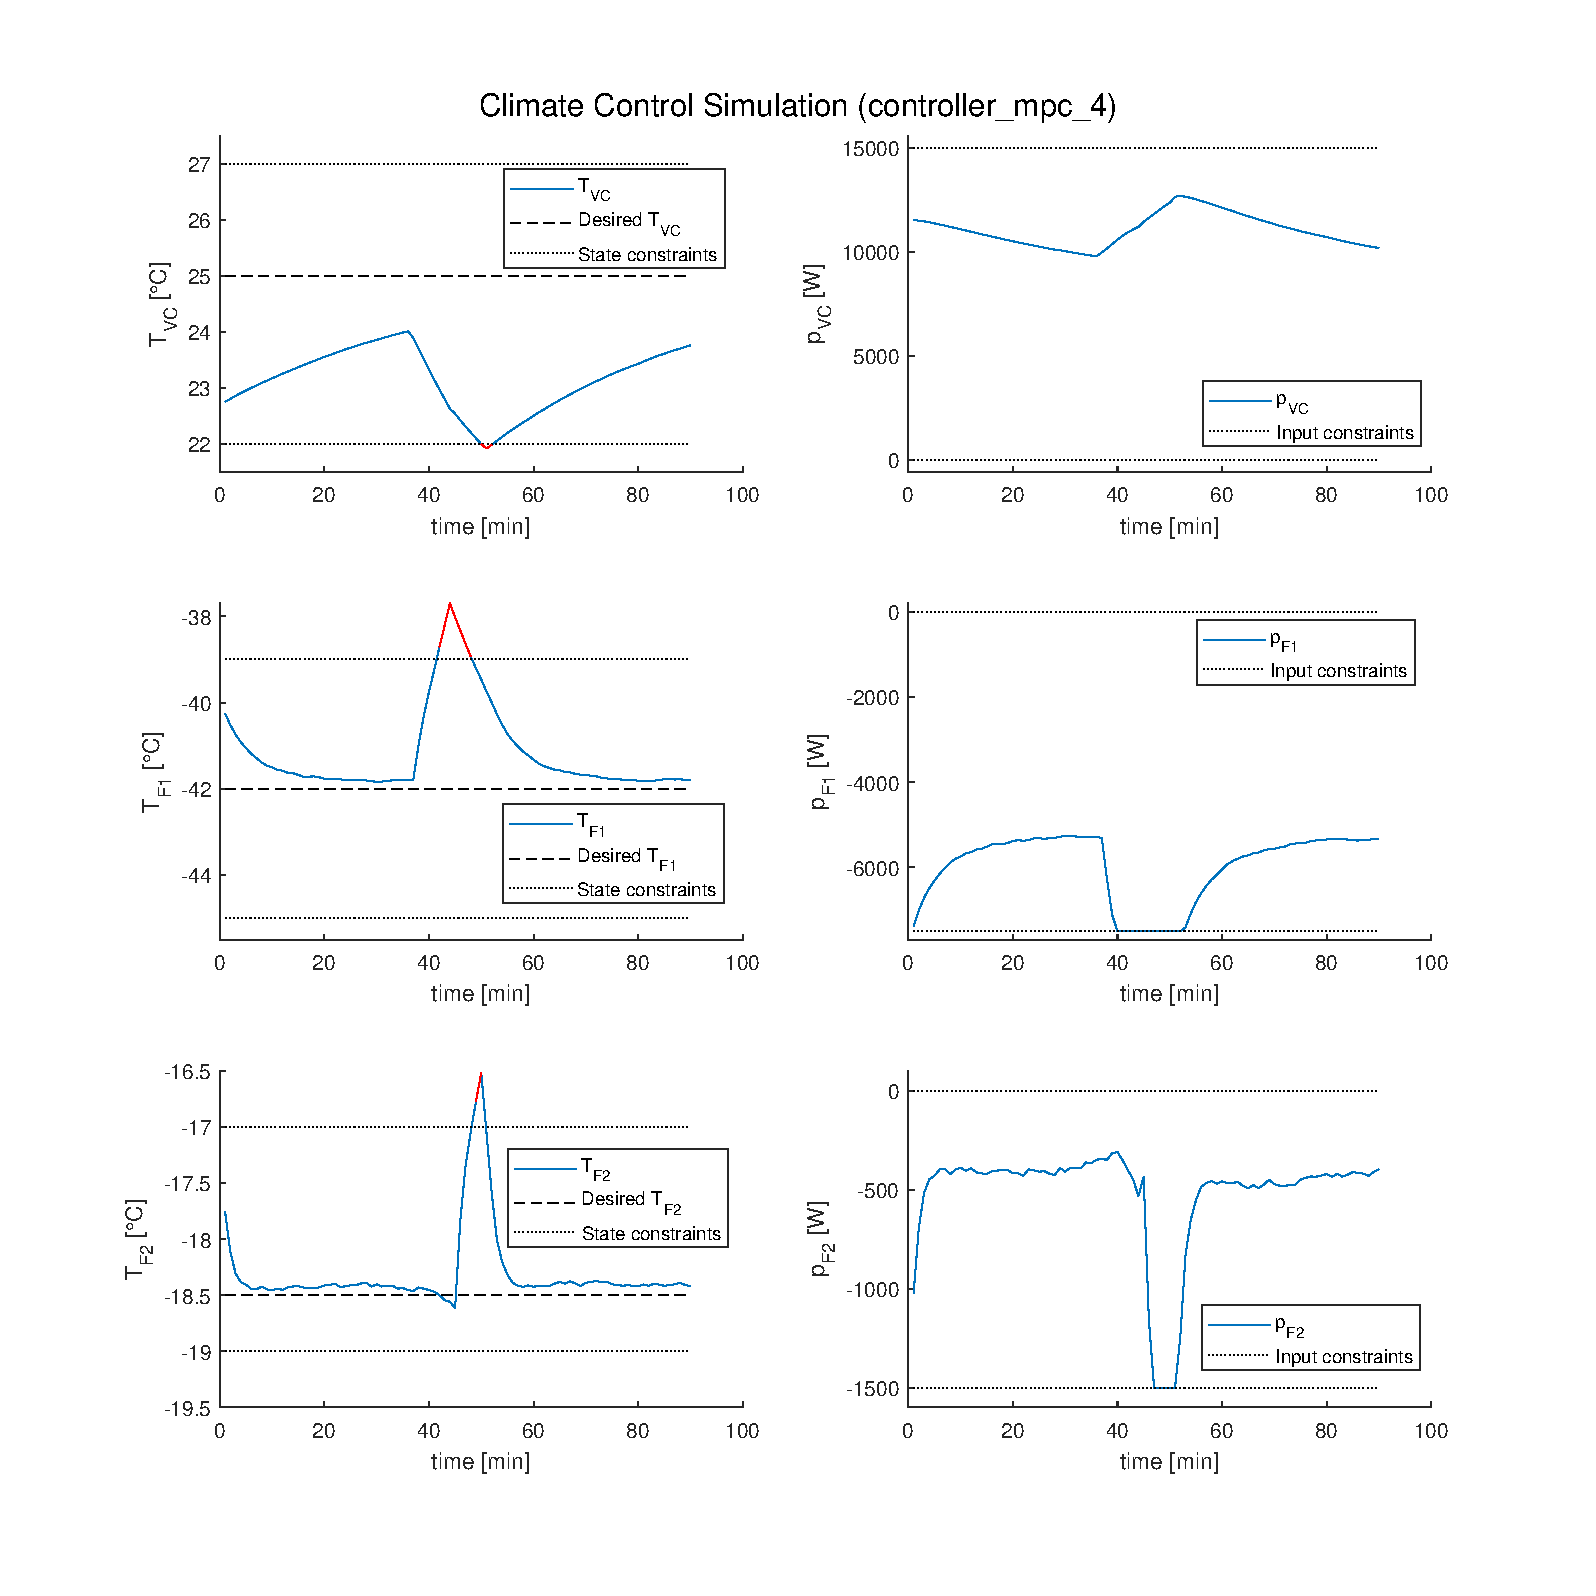
\includegraphics[scale = 0.58]{image/18.eps}
\caption{Simulation of Scenario 2 with initial condition 1 Using Soft-constrained MPC Controller}
\label{fig:16}
\end{figure}

\subsection{Task 19: Comparison of Simulation under Scenario 1 Between MPC Controller 3 and 4 (1 pt.)}

Figure \ref{fig:17} and \ref{fig:18} shows the simulation plots under scenario 1 using the nominal and soft-constrained MPC controller. They are identical and show that if the initial state is within the feasible range, the soft-constrained MPC controller will produce the same result as the nominal MPC controller, as all slack variables equal to 0.

\begin{figure}[ht]
\centering
\includegraphics[scale = 0.58]{image/19-1.eps}
\caption{Simulation under Scenario 1 Using MPC Controller}
\label{fig:17}
\end{figure}

\newpage

\begin{figure}[ht]
\centering
\includegraphics[scale = 0.58]{image/19-2.eps}
\caption{Simulation under Scenario 1 Using Soft-constrained MPC Controller}
\label{fig:18}
\end{figure}

\subsection{Task 20: Incorporate Future Disturbances into the Soft-constrained MPC Controller (2 pt.)}

Figure \ref{fig:19} shows the simulation plots under scenario 2 using the soft-constrained MPC controller with (blue) and without (other colors) future disturbance incorporation. By observing the disturbance in \verb|scen2|, we noticed that there are values at some time step whose absolute values are much larger than the rest of the values, so we decided to captures these features in the  disturbance matrix defined. 

We noticed that \verb|d_VC_scen| will have a huge decrease from 36 to 50 minutes with the expected value $-1.2\times10^{4}$, \verb|d_F1_scen| will have a huge increase from 37 to 43 minutes with the expected value $5.5\times 10^{3}$, \verb|d_F2_scen| will have a huge increase from 37 to 43 minutes with the expected value $1\times 10^{3}$. Thus, we could use the observation to define the disturbance matrix and set other values to 0. 

The MPC controller yields a even better performance since all state constraints will not be violated. The reason is mainly that in the soft-constrained MPC controller, we have a better dynamic model of the system which incorporated the expected future disturbances. As a result, the MPC controller will take the disturbances into account and yield an input that will drive the system without violating the state constraints even under the situation of disturbance. 


\begin{figure}[ht]
\centering
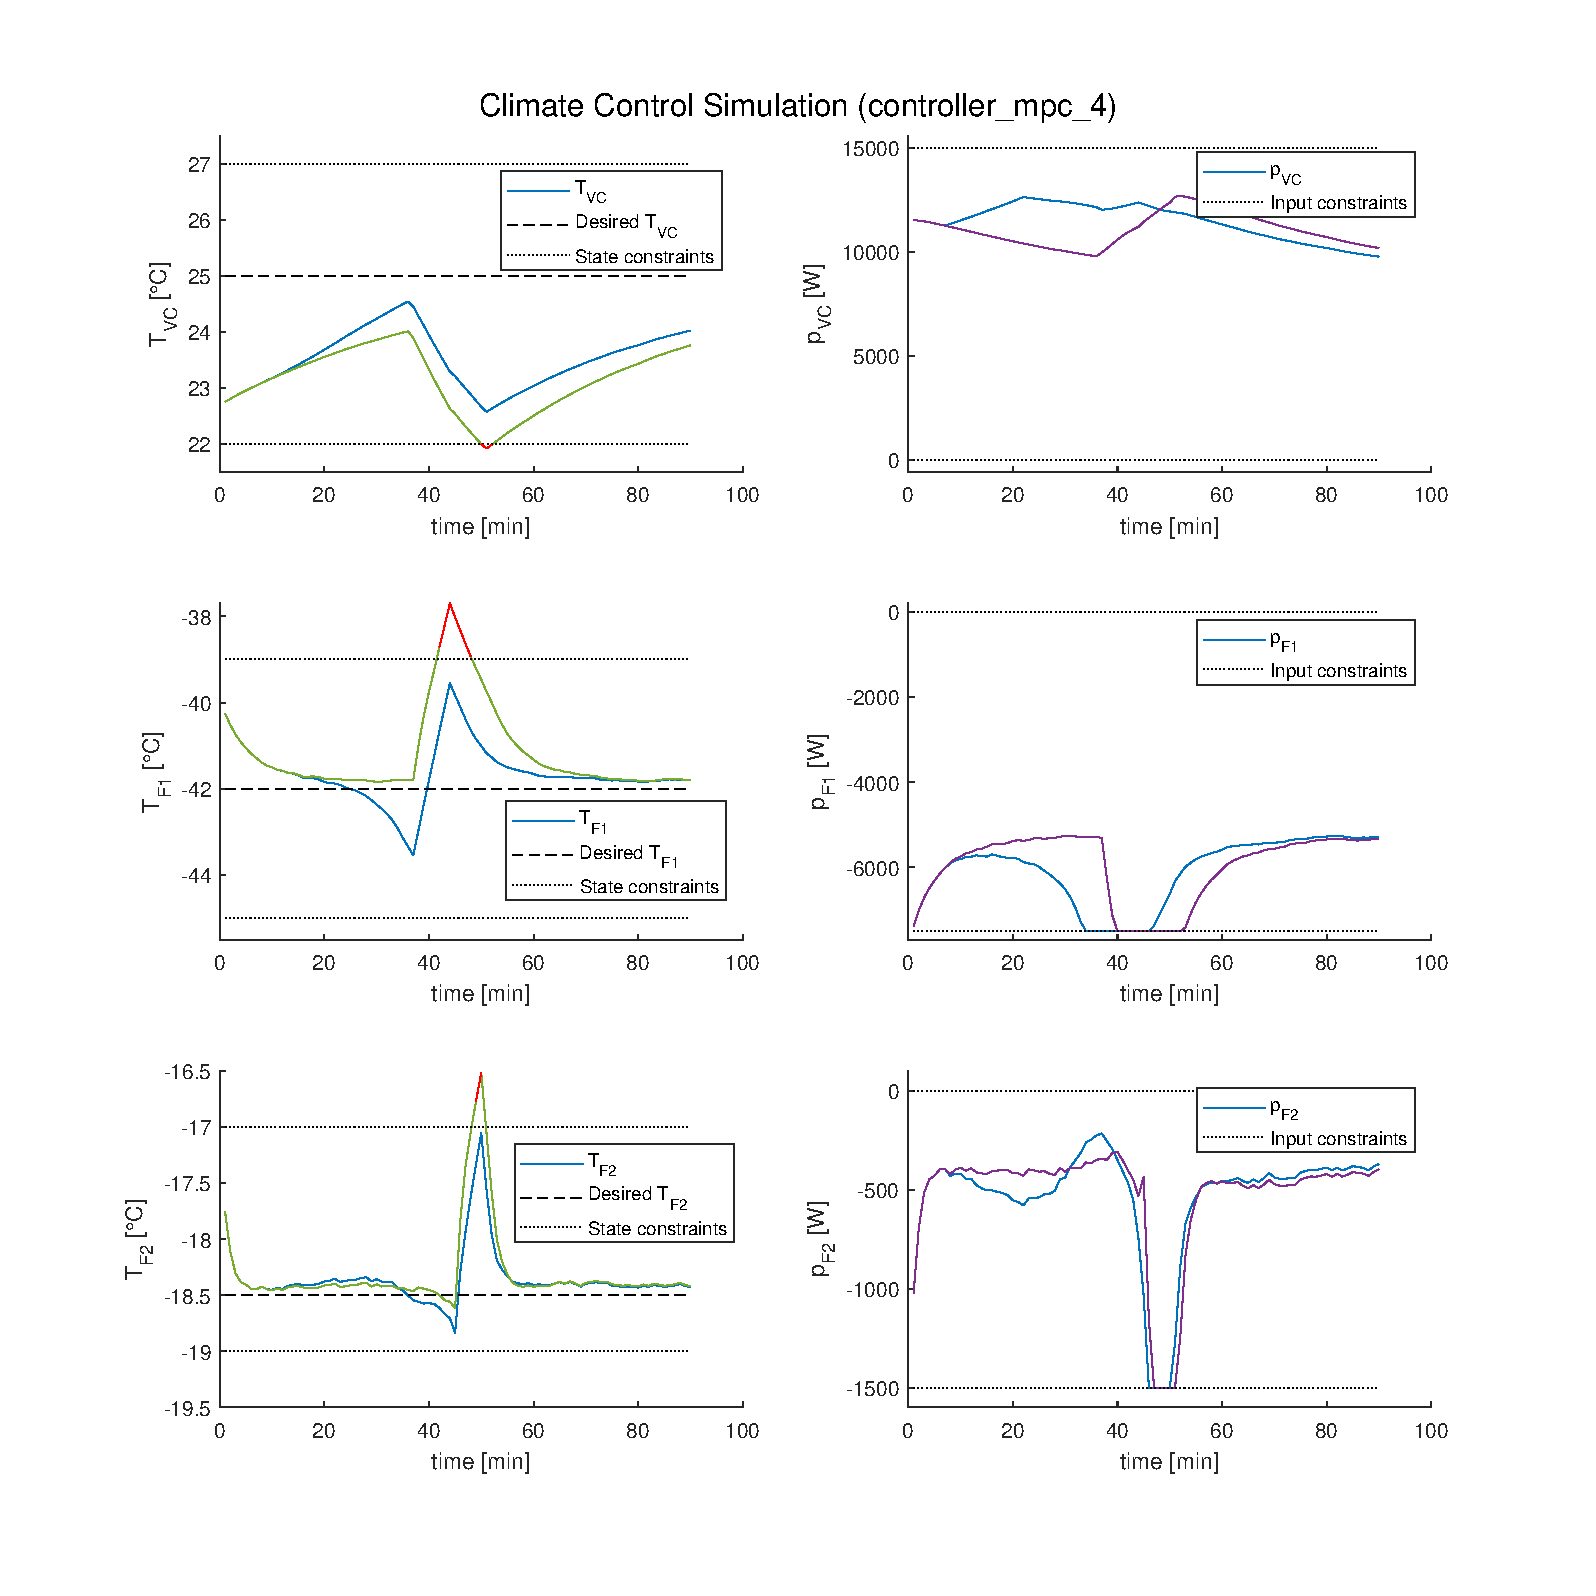
\includegraphics[scale = 0.58]{image/20.eps}
\caption{Simulation under Scenario 1 Using Soft-constrained MPC Controller with (blue) and without (other colors) Future Disturbances}
\label{fig:19}
\end{figure}

\newpage

%--------------------------------------------------------------------

\section{Offset-free MPC}

\subsection{Task 21: Augmented model (2 pt.)}

The nominal dynamics we have from the previous tasks is
\begin{equation}
    \begin{split}
        T(k+1) &= AT(k)+Bp(k)+B_d d \\
        y(k) &= T(k)
    \end{split}
\end{equation}

And here we can model the constant disturbance $\Bar{d}$ as a variable so that it can be observed. 
\begin{equation}
    \begin{split}
        T(k+1) &= AT(k)+Bp(k)+B_d d(k) \\
        d(k+1) &= d(k) \\
        y(k) &= T(k)
    \end{split}
\end{equation}

By reformulating it, we have
\begin{equation}
    \begin{split}
        \begin{bmatrix}
        T(k+1) \\
        d(k+1)
        \end{bmatrix}
        &=A_{aug}
        \begin{bmatrix}
        T(k) \\
        d(k)
        \end{bmatrix}
        +
        B_{aug}p(k) \\
        y(k) &=
        C_{aug}
        \begin{bmatrix}
        T(k) \\
        d(k)
        \end{bmatrix}
        + D_{aug}p(k)
    \end{split}
\end{equation}

where 
\begin{equation*}
    A_{aug} = \begin{bmatrix}
    A & B_d \\
    0 & I
    \end{bmatrix}, 
    B_{aug} = \begin{bmatrix}
    B \\
    0
    \end{bmatrix}, 
    C_{aug} = \begin{bmatrix}
    I & 0
    \end{bmatrix}, 
    D_{aug} = 0
\end{equation*}


\subsection{Task 22: The Linear Observer Design (2 pt.)}

The linear observer will take the form 
\begin{equation}
    \begin{bmatrix}
    \hat{T}(k+1)\\
    \hat{d}(k+1)
    \end{bmatrix}
    = A_{aug}
    \begin{bmatrix}
    \hat{T}(k)\\
    \hat{d}(k)
    \end{bmatrix}
    + B_{aug}p(k)
    + L\left(y(k)-C_{aug}\begin{bmatrix}
    \hat{T}(k)\\
    \hat{d}(k)\end{bmatrix}\right)
\end{equation}

The error dynamics is
\begin{equation}
    \begin{split}
        \begin{bmatrix}
        T(k+1)-\hat{T}(k+1)\\
        d(k+1)-\hat{d}(k+1)
        \end{bmatrix}
        &=
        A_{aug}
        \begin{bmatrix}
        T(k)-\hat{T}(k)\\
        d(k)-\hat{d}(k)
        \end{bmatrix}
        -LC_{aug}
        \begin{bmatrix}
        T(k)-\hat{T}(k)\\
        d(k)-\hat{d}(k)
        \end{bmatrix} \\
        &=
        (A_{aug}-LC_{aug})
        \begin{bmatrix}
        T(k)-\hat{T}(k)\\
        d(k)-\hat{d}(k)
        \end{bmatrix}
    \end{split}
\end{equation}

Here our goal is to choose $L$ such that the error dynamics are stable and converge to zero. Thus, we use the \verb|place()| function in MATLAB to place the eigenvalues of $A_{aug}-LC_{aug}$ to $[0.8, 0.8, 0.8, 0.0, 0.0, 0.0]$. 

Using the steady state condition we have
\begin{equation}
    T_s = T_{Target}
\end{equation}
\begin{equation}
    T_s = AT_s + Bp_s +B_d \hat{d}
\end{equation}

where $\hat{d}$ is the current estimation of disturbance, which is also the best forecast for steady state disturbance. $T_{Target} = [25, -42, -18.5]^\top$ is the constant reference we want to track.

It is easy to reformulate it as

\begin{equation}
    \begin{bmatrix}
    A-I & B \\
    I & 0
    \end{bmatrix}
    \begin{bmatrix}
    T_s \\
    p_s
    \end{bmatrix}
    =
    \begin{bmatrix}
    -B_d \hat{d} \\
    T_{Target}
    \end{bmatrix}
\end{equation}


\subsection{Task 23: Simulation Using the Offset-free MPC Controller (6 pt.)}

At each time step, we need to first estimate the state $\hat{T}(k)$ and disturbance $\hat{d}(k)$ using the linear observer, and then compute the steady-state $T_s$ and its input $p_s$ based on the estimated disturbance $\hat{d}(k)$ as shown in the previous question. And here we denote
\begin{equation*}
    x(k) = \Delta T(k) = T(k) - T_s
\end{equation*}
\begin{equation*}
    u(k) = \Delta p(k) = p(k) - p_s
\end{equation*}

The system dynamics will be
\begin{equation}
    x(k+1) = Ax(k) + Bu(k)
\end{equation}

Then the Offset-free Tracking MPC problem will be like
\begin{equation}
\begin{split}
    min_U & \sum_{i=0}^{N-1}x_i^\top Q x_i+u_i^\top R u_i + I_f(x_{N}) \\
    s.t. \quad & x_0 = \hat{x}(k) = \hat{T}(k) - T_s \\
    & d_0 = \hat{d}(k) \\
    & x_{i+1} = Ax_i + Bu_i + B_d d_i \\
    & d_{i+1} = d_i \\
    & x_{min} \le x_i \le x_{max} \\
    & u_{min} \le u_i \le u_{max} \\
    & x_N \in X_{LQR}
\end{split}
\end{equation}

Figure \ref{fig:20} and \ref{fig:21} show the simulation plot under scenario 3 using offset-free MPC controller and the vanilla MPC controller (MPC controller 3). 

When dealing with unknown but almost constant disturbance, the offset-free MPC controller will have a much better performance. We can observe that the temperatures in the vaccinations will converge really soon and the convergence of the building temperature is not affected by the disturbance. However, the vanilla MPC controller can not drive the system converge to the reference temperatures without offset. This is mainly because the system model implemented in the vanilla MPC controller is not accurate in the lack of disturbance. 

\newpage

\begin{figure}[ht]
\centering
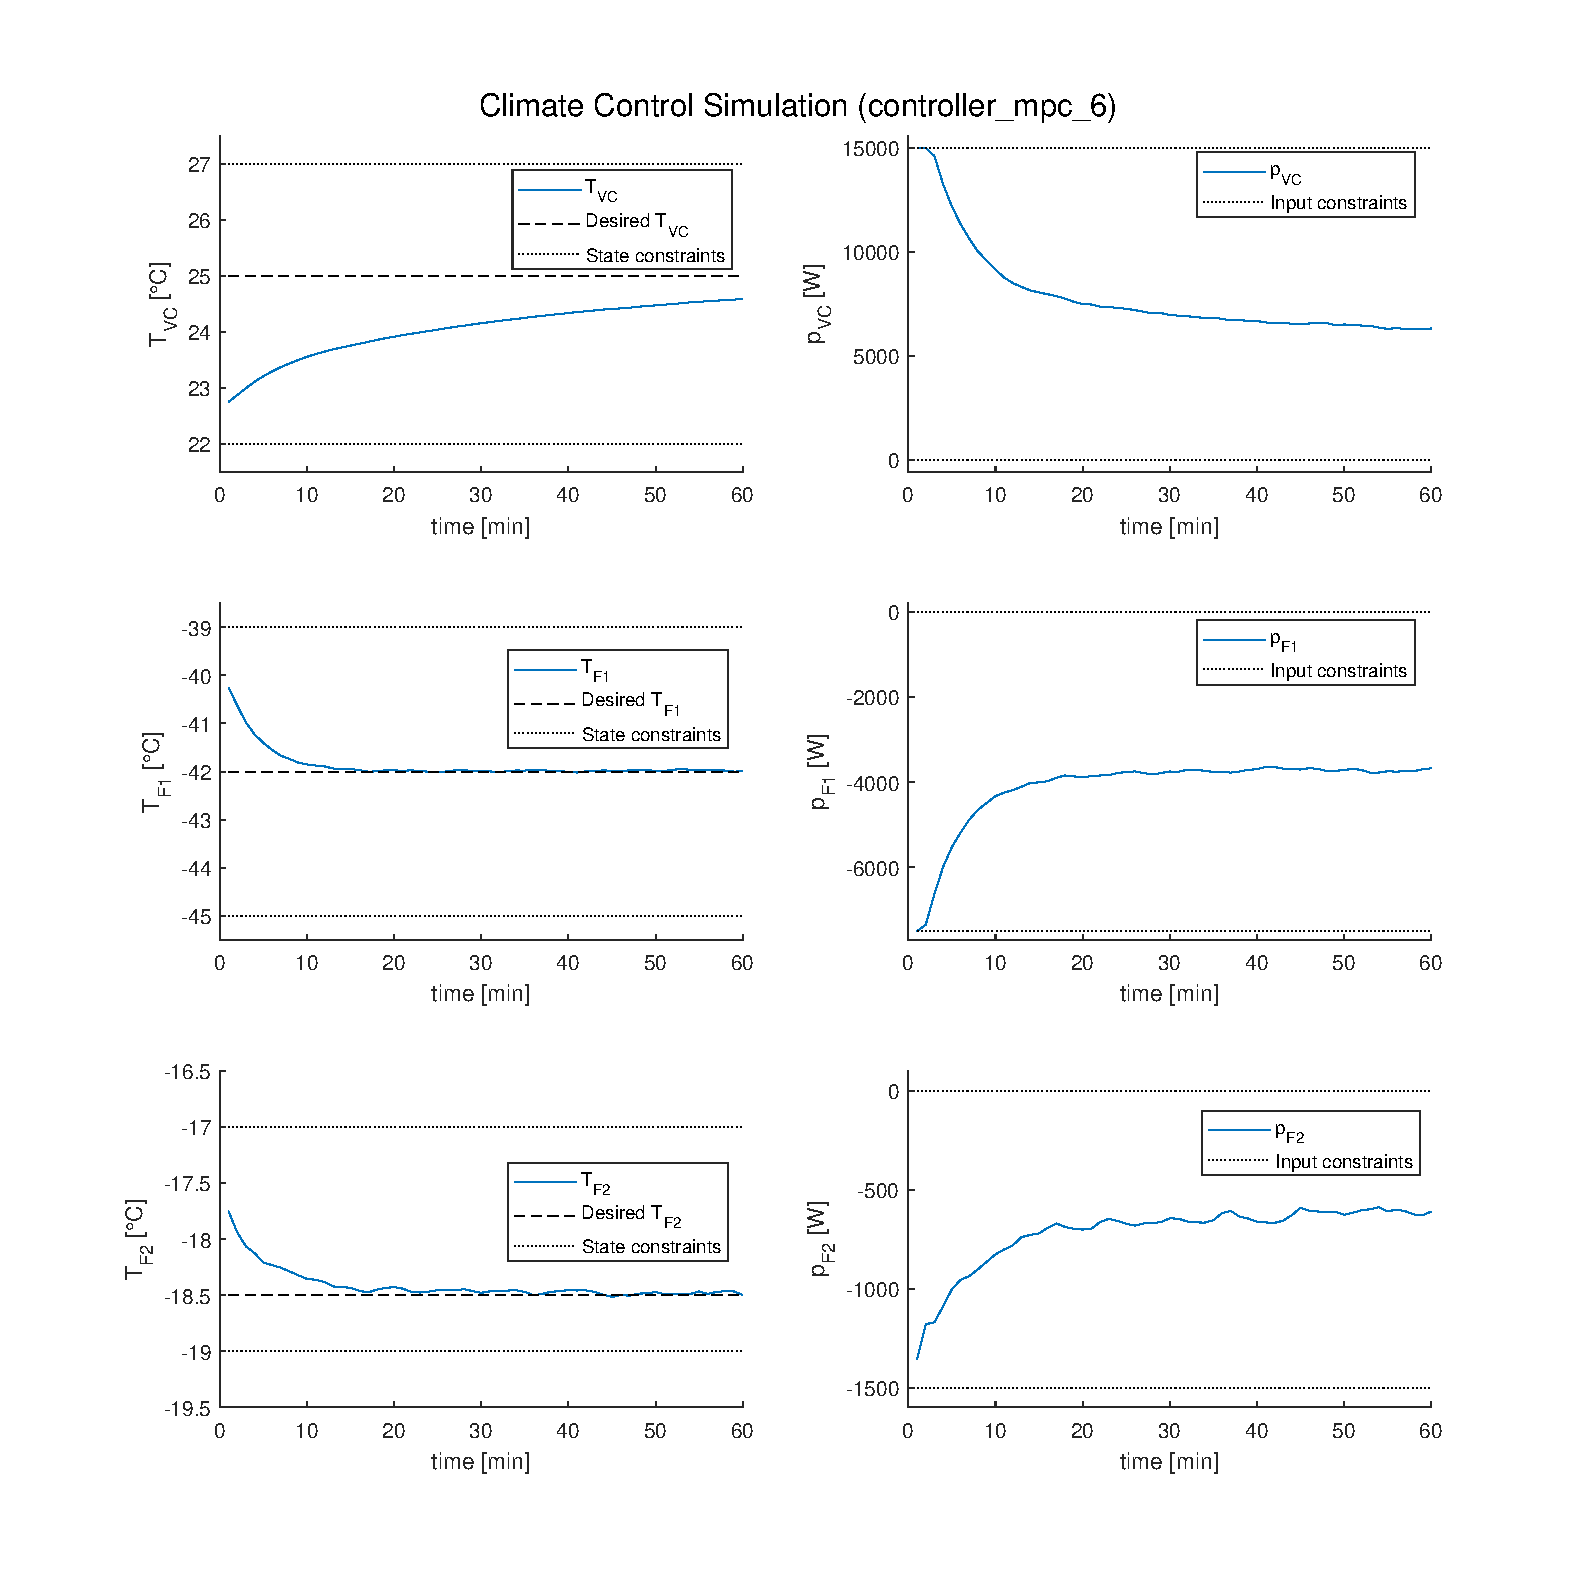
\includegraphics[scale = 0.58]{image/23-1.eps}
\caption{Simulation Under Scenario 3 Using Offset-free MPC Controller}
\label{fig:20}
\end{figure}

\newpage

\begin{figure}[ht]
\centering
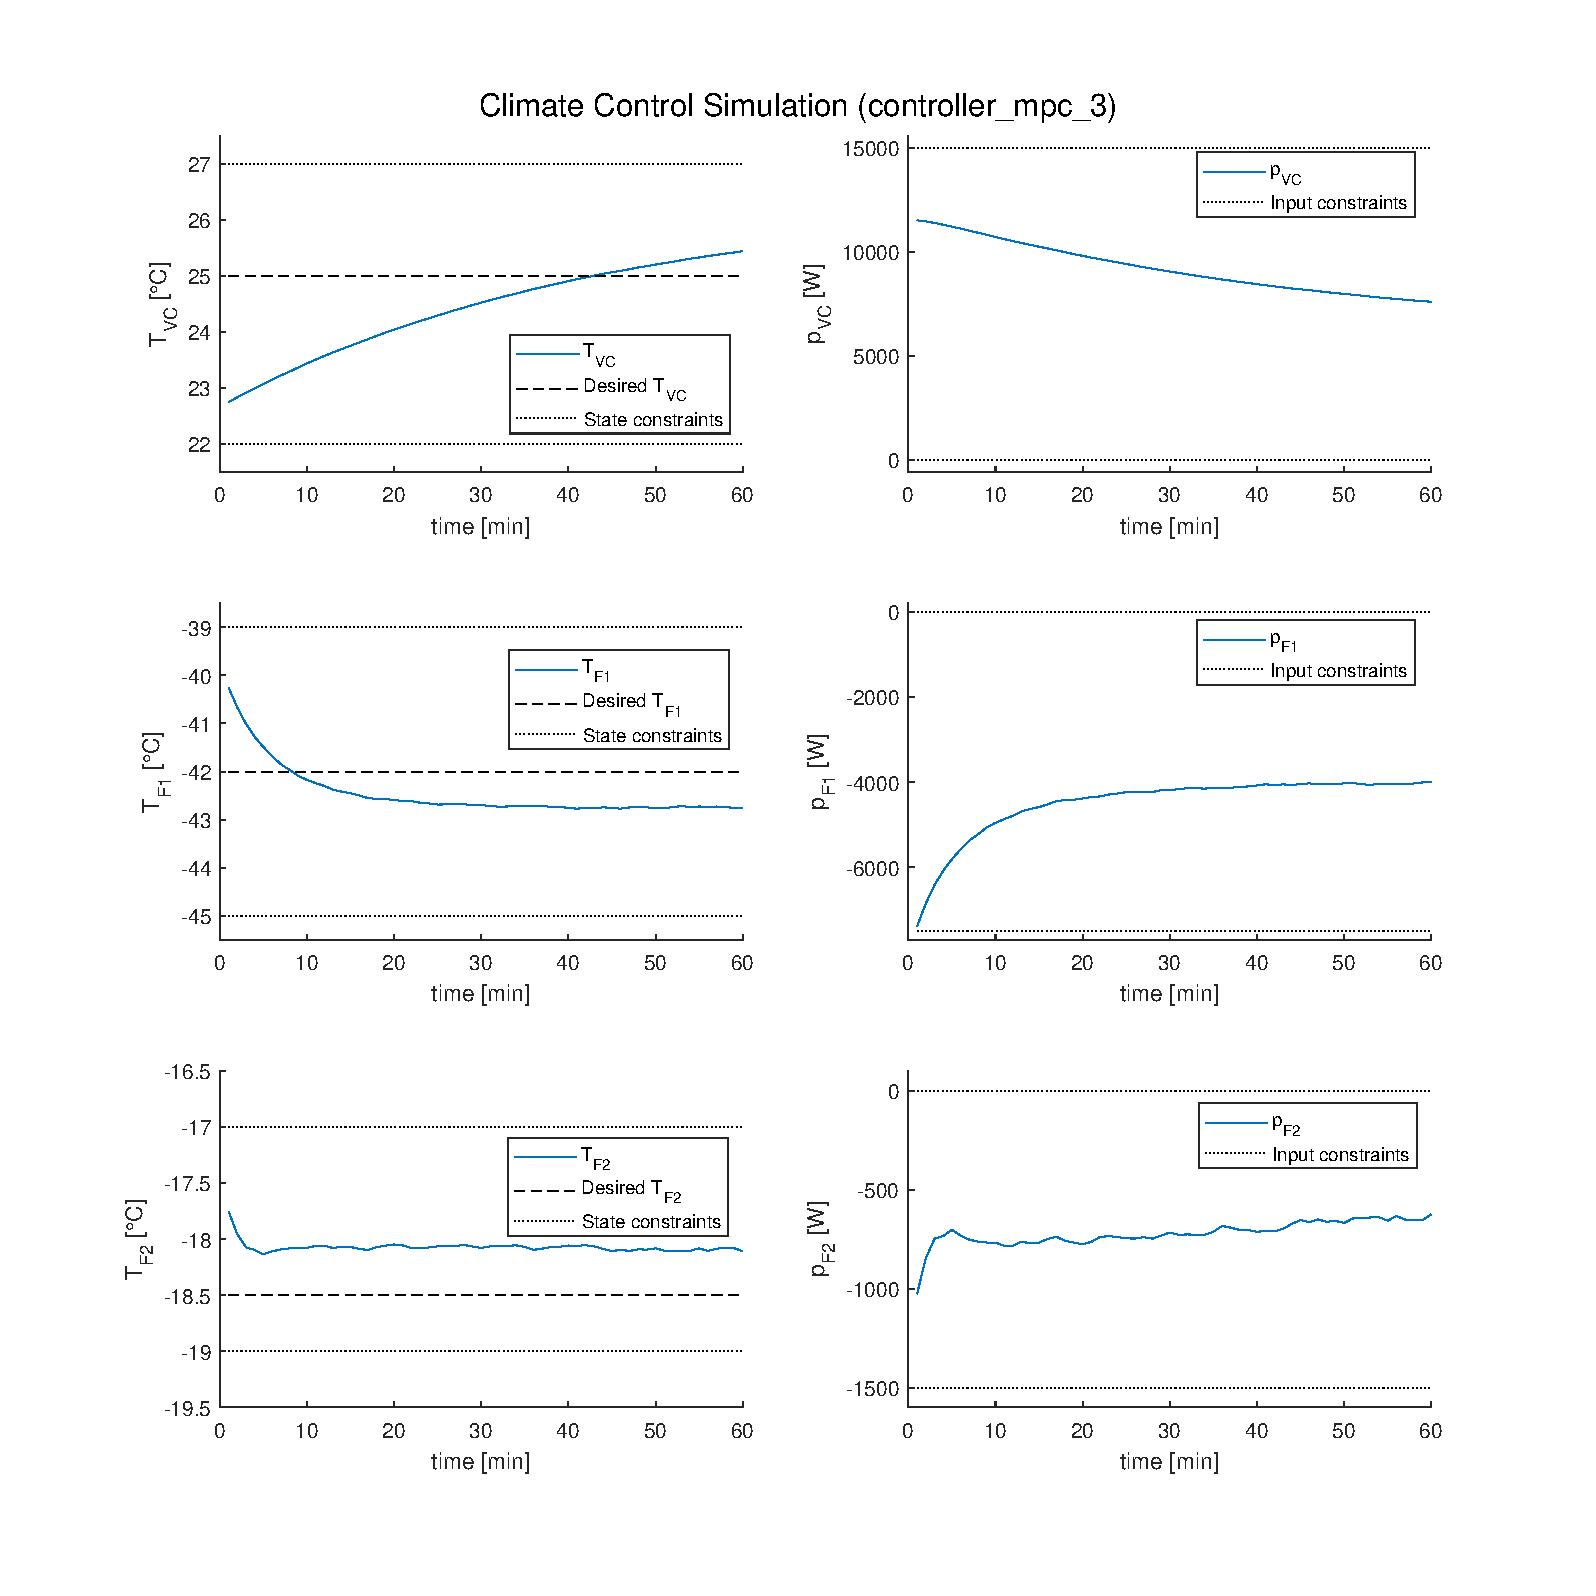
\includegraphics[scale = 0.58]{image/23-2.eps}
\caption{Simulation Under Scenario 3 Using Vanilla MPC Controller}
\label{fig:21}
\end{figure}

\newpage

%-----------------------------------------------------------------

\section{FORCES Pro}

\subsection{Task 24: MPC Implementation with FORCES Pro (3 pt.)}


We can simply change the \verb|optimizer()| to \verb|optimizerFORCES()|, and modify the solver options to implement the FORCES Pro solver. By running the simulation under scnenario 1 with initial condition 2 using MPC controller 1, we can get the running times for the controllers. 

The controller 1 using FORCES Pro will have running time 0.078119 s, while the original controller will have running time 1.645772 s. It is obvious that the controller using FORCES Pro is extremely faster than that using the MATLAB implemented optimizer. 

\end{document}
